% `advanced_example.tex', an advanced example employing the AIAA class
% plus other third-party LaTeX packages.
%
% For a bare-bones usage, see `template.tex'.
%
% Typical processing for PostScript (PS) output:
%
%  latex advanced_example
%  bibtex advanced_example  (bibliography)
%  makeindex -s nomencl.ist -o advanced_example.gls advanced_example.glo
%                            (nomenclature)
%  latex advanced_example   (repeat as needed to resolve references)
%
%  xdvi advanced_example    (onscreen draft display)
%  dvips advanced_example   (postscript)
%  gv advanced_example.ps   (onscreen display)
%  lpr advanced_example.ps  (hardcopy)
%
% With the above, only Encapsulated PostScript (EPS) images can be used.
%
%
%  pdflatex advanced_example
%  bibtex advanced_example    (bibliography)
%  makeindex -s nomencl.ist -o advanced_example.gls advanced_example.glo
%                              (nomenclature)
%  pdflatex advanced_example  (repeat as needed to resolve references)
%
%  acroread advanced_example.pdf  (onscreen display)
%
% If you have EPS figures, you will need to use the epstopdf script
% to convert them to PDF because PDF is a limmited subset of EPS.
% pdflatex accepts a variety of other image formats such as JPG, TIFF,
% PNG, and so forth -- check the documentation for your version.
%
% If you do *not* specify suffixes when using the graphicx package's
% \includegraphics command, latex and pdflatex will automatically select
% the appropriate figure format from those available.  This allows you
% to produce PS and PDF output from the same LaTeX source file.
%
% To generate a large format (e.g., 11"x17") PostScript copy for editing
% purposes, use
%
%  dvips -x 1467 -O -0.65in,0.85in -t tabloid advanced_example
%
% For further details and support, read the Users Manual, aiaa.pdf.

\documentclass[]{aiaa-tc}% insert '[draft]' option to show overfull boxes

 \usepackage{varioref}%  smart page, figure, table, and equation referencing
 \usepackage{wrapfig}%   wrap figures/tables in text (i.e., Di Vinci style)
 \usepackage{threeparttable}% tables with footnotes
 \usepackage{dcolumn}%   decimal-aligned tabular math columns
  \newcolumntype{d}{D{.}{.}{-1}}
 \usepackage{nomencl}%   nomenclature generation via makeindex
  \makeglossary
 \usepackage{amssymb,amsmath}
 \usepackage{subfigure}% subcaptions for subfigures
 \usepackage{subfigmat}% matrices of similar subfigures, aka small mulitples
 \usepackage{fancyvrb}%  extended verbatim environments
 \fvset{fontsize=\footnotesize,xleftmargin=2em}
 \usepackage{lettrine}%  dropped capital letter at beginning of paragraph
%  \usepackage[dvips]{dropping}% alternative dropped capital package
 \usepackage[colorlinks]{hyperref}%  hyperlinks [must be loaded after dropping]
 \usepackage{float}
 \usepackage{longtable,booktabs,tabularx}
 \restylefloat{table}
 \usepackage{graphicx}
 \usepackage{caption}
 \usepackage{siunitx}
 \usepackage{multicol}
 \usepackage{indentfirst}
 \usepackage[labelfont=bf]{caption}
 \usepackage{multirow}
 \usepackage{setspace}
 \usepackage[sort, numbers]{natbib}
 \doublespacing

 \title{Solar-Electric and Gas Powered, Long-Endurance UAV Sizing via Geometric Programming}

 \author{
  Michael Burton \thanks{Master's Candidate, Aeronautics and Astronautics Engineering, 77 Mass Ave, Cambridge MA, 02139, AIAA Student.}
  \ and Warren Hoburg\thanks{Assistant Professor, Aeronautics and Astronautics Engineering, 77 Mass Ave, Cambridge MA, 02139, AIAA Member.}\\
  {\normalsize\itshape
   Massachusetts Institute of Technology, Cambridge, 02139, USA}\\
 }

 % Data used by 'handcarry' option
 \AIAApapernumber{YEAR-NUMBER}
 \AIAAconference{Conference Name, Date, and Location}
 \AIAAcopyright{\AIAAcopyrightD{YEAR}}

 % Define commands to assure consistent treatment throughout document
 \newcommand{\eqnref}[1]{(\ref{#1})}
 \newcommand{\class}[1]{\texttt{#1}}
 \newcommand{\package}[1]{\texttt{#1}}
 \newcommand{\file}[1]{\texttt{#1}}
 \newcommand{\BibTeX}{\textsc{Bib}\TeX}
 \usepackage{hyperref}
 \hypersetup{citecolor = blue}

\begin{document}

\maketitle

\begin{abstract}
    Fueled by telecommunication needs and opportunities, there has been a recent push to develop aircraft that can provide long-endurance (days to weeks) persistent aerial coverage.
    These aircraft present a complicated systems engineering problem because of the multifaceted interaction of various requirements, such as endurance, wind speeds, operational capability and coverage footprint.
    In this paper, a comparison of solar-electric and gas powered, long-endurance aircraft is accomplished.
    Geometric programming, a form of convex optimization, can reliably solve problems with thousands of variables in seconds and is used as an optimization tool to evaluate the design trade offs between architectures and requirements.
    The results show that long-endurance, gas powered aircraft are generally more robust to higher wind speeds than solar-powered aircraft.  
    However, gas powered aircraft are limited in their endurance by the amount of fuel that they can carry. 
    While solar-electric powered aircraft can theoretically fly for months, they are operationally limited by reduced solar flux during the winter and wind speeds at higher latitudes.
    Using geometric programming, a detailed trade study between gas-powered and solar-powered aircraft is performed to discover which architecture is best suited to meet a given set of requirements, and what is the optimum size and endurance of that platform.
\end{abstract}

\section*{Nomenclature}

\begin{multicols}{2}
\small

\begin{tabbing}
  XXXXXXX \= \kill% this line sets tab stop
$A$ \> wing aspect ratio \\
$\bar{A}$ \> non-dimensional cross sectional area \\
$b$ \> wing span \\ % [ft] \\
BSFC \> brake specific fuel consumption \\ %[kg/kW/hr] \\
$\text{BSFC}_{100\%}$ \> BSFC at full throttle \\ %[kg/kW/hr] \\
$c$ \> wing chord \\ %[m] \\
$C_D$ \> aircraft drag coefficient \\
$C_{d_0}$ \> non-wing drag coefficient \\
$c_{d_{\text{h}}}$ \> horizontal tail profile drag coefficient \\
$c_{d_p}$ \> wing profile drag coefficient \\
$c_{d_{\text{v}}}$ \> vertical tail profile drag coefficient \\
$C_f$ \> skin friction coefficient \\
$C_L$ \> lift coefficient \\
$c_{l_{\alpha}}$ \> lift slope coefficient \\
$C_{L_{\text{max}}}$ \> maximum lift coefficient \\
$d$ \> tail boom diameter \\ %[m] \\
$D_{\text{boom}}$ \> tail boom drag \\% [N] \\
$\Delta W$ \> wing section weight \\ %[N] \\
$\Delta y$ \> wing section length \\ %[m] \\
DOY \> day of the year \\
$e$ \> Oswald efficiency factor \\
$E$ \> Young's Modulus \\ %[Pa] \\
$E_{\text{batt}}$ \> energy stored in battery \\ %[J] \\
$E_{\text{sun}}$ \> total solar energy available \\ %[Whr] \\
$(E/S)_{\text{twilight}}$ \> twilight solar energy \\ %[Whr/m$^2$] \\
$(E/S)_{\text{day}}$ \> daily required solar energy \\ % [Whr/m$^2$] \\
$(E/S)_{\text{sun}}$ \> available solar energy \\ % [Whr/m$^2$] \\
$f_{\text{solar}}$ \> planform area fraction covered in solar cells \\
$f_{\text{structural}}$ \> fractional structural weight\\
$g$ \> gravitational constant \\ % [m/s$^2$] \\
$h$ \> flight altitude \\ % [ft] \\
$h_{\text{batt}}$ \> battery specific energy \\ % [Whr/kg] \\
$h_{\text{cap}}$ \> spar cap separation \\ % [m] \\
$I$ \> cap spar moment of inertia \\ % [m$^4$] \\
$I_0$ \> tail boom root moment of inertia \\ % [m$^4$] \\
$k$ \> tail boom taper index \\
$K_q$ \> wing loading constant \\ % [N/m$^2$] \\
$L$ \> atmospheric lapse rate \\ % [K/m] \\
$L_\text{h}$ \> horizontal tail lift \\ % [N] \\
$l_\text{fuse}$ \> fuselage length \\ % [m] \\
$l_\text{h}$ \> horizontal tail moment arm \\ % [m] \\
$l_\text{v}$ \> vertical tail moment arm \\ % [m] \\
$m$ \> tail boom mass \\ % [kg] \\
$m'$ \> local wing mass \\ % [kg/m] \\
$m_{\text{fac-wing}}$ \> margin factor\\
$m_{\text{fac-wing}}$ \> wing weight margin factor \\
$m_{\text{motor}}$ \> electric motor mass \\
$\dot{m}_{\text{fuel}}$ \> fuel flow rate \\ % [kg/s] \\
$\mathcal{M}$ \> wing bending moment \\ % [Nm] \\
MTOW \> max take-off weight \\ % [N] \\
$n$ \> number of wing segments \\
$N$ \> number of flight segments \\
$N_{\text{max}}$ \> safety load factor\\
$p$ \> air pressure \\ % [Pa]\\
$p_{11}$ \> air pressure at 11,000 meters \\ % [Pa]\\
$p_{\text{wind}}$ \> percentile wind speed \\
$P_{0}$ \> magnitude of available solar power \\ % [W/m$^2$] \\
$P_{\text{avionics}}$ \> avionics power \\ % [hp] \\
$P_{\text{oper}}$ \> aircraft operating power \\ % [hp] \\
$(P/S)_{\text{min}}$ \> minium operational solar power \\ % [Whr/m$^2$] \\
$P_{\text{shaft}}$ \> engine/motor shaft power \\ % [hp] \\
$P_{\text{sun}}$ \> useable solar power per unit area \\ % [W/m$^2$] \\
$P_{\text{sun surface}}$ \> power emitted at the sun's surface \\ % [W/m$^2$] \\
$r_0$ \> average distance from earth to sun \\
$R$ \> aircraft range \\ % [nmi] \\
$R_{\text{earth orbit}}$ \> distance from earth to sun \\
$R_{\text{fuse}}$ \> fuselage radius \\ % [m] \\
$R_{\text{spec}}$ \> specific gas constant \\ % [J/k/K] \\
$R_{\text{sun}}$ \> radius of the sun \\
$q$ \> distributed wing loading \\ % [N/m] \\
$\bar{q}$ \> normalized distributed wing loading \\
$Re$ \> aircraft Reynolds number \\
$Re_{\text{boom}}$ \> tail boom Reynolds number \\
$Re_{\text{h}}$ \> horizontal tail Reynolds number \\
$Re_{\text{v}}$ \> vertical tail Reynolds number \\
$S$ \> wing planform area \\ % [m$^2$]\\
$\mathcal{S}$ \> shear forces \\ % [N] \\
$S_{\text{fuse}}$ \> fuselage wetted surface area \\ % [m$^2$]\\
$S_{\text{h}}$ \> horizontal tail planform area \\ % [m$^2$]\\
$S_{\text{solar}}$ \> solar cell area \\ % [m$^2$]\\
$S_{\text{v}}$ \> vertical tail planform area \\ % [m$^2$]\\
$t$ \> flight time \\ % [days] \\
$t_0$ \> tail boom root wall thickness \\ % [m] \\
$t_{\text{cap}}$ \> spar cap thickness \\ % [m] \\
$t_{\text{day}}$ \> hours of daylight \\ % [hr] \\
$t_{\text{night}}$ \> hours of darkness \\ % [hr] \\
$t_{\text{sun rise}}$ \> time of sun rise \\ % [hr] \\
$t_{\text{sun set}}$ \> time of sun set \\ % [hr] \\
$T$ \> aircraft thrust \\ % [N] \\
$T_{11}$ \> air temperature at 11,000 meters \\ % [K] \\
$T_{\text{atm}}$ \> air temperature at flight altitude \\ % [K] \\
$T_{\text{sl}}$ \> air temperature at sea level \\ % [K] \\
$V$ \> true airspeed \\ % [m/s] \\
$\mathcal{V}_{\text{fuse}}$ \>  fuselage volume \\ % [m$^3$] \\
$V_{\text{gust}}$ \>  gust velocity \\ % [m/s] \\
$V_{\text{h}}$ \> horizontal tail lift coefficient \\
$V_{\text{ref}}$ \>  reference wind airspeed \\ % [m/s] \\
$V_{\text{wind}}$ \>  wind speed \\ % [m/s] \\
$V_{\text{v}}$ \> vertical tail lift coefficient \\
$w$ \> wing deflection \\ % [m] \\
$W$ \> aircraft weight \\ % [N] \\
$W_{\text{ave}}$ \> average weight over a flight segment \\ % [N] \\
$W_{\text{batt}}$ \> battery weight \\ % [N] \\
$w_{\text{cap}}$ \> spar cap width \\ % [m] \\
$W_{\text{cent}}$ \> center of aircraft weight \\ % [N] \\
$W_{\text{empennage}}$ \> empennage weight \\ % [N] \\
$W_{\text{engine}}$ \> engine weight \\ % [N] \\
$W_{\text{final}}$ \> end of flight segment aircraft weight \\ % [N] \\
$W_{\text{fuel}}$ \> fuel weight \\ % [N] \\
$W_{\text{fuselage}}$ \> fuselage weight \\ % [N] \\
$W_{\text{h}}$ \> horizontal tail weight \\ % [N] \\
$W_{\text{initial}}$ \> start of flight segment aircraft weight \\ % [N] \\
$w_{\text{max}}$ \> maximum deflection limit \\ % [m] \\
$W_{\text{payload}}$ \> payload weight \\ % [N] \\
$W_{\text{skin}}$ \> wing skin weight \\ % [N] \\
$W_{\text{solar}}$ \> solar cell weight \\ % [N] \\
$W_{\text{spar}}$ \> wing spar weight \\ % [N] \\
$W_{\text{structural}}$ \> structural weight \\ % [N] \\
$W_{\text{v}}$ \> vertical tail weight \\ % [N] \\
$W_{\text{wing}}$ \> wing weight \\ % [N] \\
$y$ \> distance from wing root along span \\ % [m] \\
$z_{\text{bre}}$ \> Breguet Range helper variable \\
$\alpha$ \> angle of attack \\
$\alpha_{\text{gust}}$ \> local angle of attack from gust velocities \\ % [rad] \\
$\Delta$ \> solar declination angle \\
$\eta_{\text{charge}}$ \> battery charging efficiency \\
$\eta_{\text{discharge}}$ \> battery discharging efficiency \\
$\eta_{\text{motor}}$ \> electric motor efficiency \\
$\eta_{\text{prop}}$ \> propulsive efficiency \\
$\eta_{\text{solar}}$ \> solar cell efficiency \\
$\mu$ \> air viscosity \\ % [kg/m/s] \\
$\mu_0$ \> reference air viscosity \\ % [kg/m/s] \\
$\phi$ \> latitude \\
$\rho$ \> air density \\ % [kg/m$^3$] \\
$\rho_{A_{\text{cfrp}}}$ \> area density of carbon fiber \\ % [kg/cm$^2$] \\
$\rho_{\text{cfrp}}$ \> density of carbon fiber \\ % [kg/cm$^3$] \\
$\rho_{\text{foam}}$ \> density of foam \\ % [lbf/ft$^3$] \\
$\rho_{\text{solar}}$ \> solar cell density \\ % [kg/m$^2$] \\
$\sigma_{\text{cfrp}}$ \> maximum carbon fiber stress \\ % [Pa] \\
$\tau_{\text{h}}$ \> horiztonal tail thickness to chord ratio \\
$\tau_t$ \> wing thickness to chord ratio \\
$\tau_{\text{v}}$ \> vertical tail thickness to chord ratio \\
$\tau_w$ \> cap spar width to chord ratio \\
$\theta$ \> angle normal to surface \\
$\theta_{\text{boom}}$ \> tail boom deflection angle \\
$\Theta$ \> wing bending deflection angle 
 \end{tabbing}

\end{multicols}
% \printglossary% creates nomenclature section produced by MakeIndex

\section{Introduction}

Long-endurance station-keeping aircraft are potential solutions to providing internet, communication, and persistent surveillance. 
Recently, tech companies such as Google\cite{googletitan} and Facebook\cite{aquila} have explored the possibility of using solar-electric powered aircraft to provide internet to parts of the world where 4G or 3G network is not available. 
Engineering firms like Aurora Flight Sciences\cite{orion} and Vanilla Aircraft\cite{vanilla} have developed gas powered long-endurance platforms as a means of providing continual surveillance for days at a time.  
Sizing of such long-endurance aircraft is complicated because of the multifaceted interaction between aerodynamics, structural weight, solar energy, wind speed, and other disciplines and environmental models.
Additionally, because few long-endurance gas and solar-electric powered aircraft have been built, the operational limits of these aircraft are relatively unknown. 
Even more unclear are the trade offs between gas powered and solar-electric powered architectures. 

This paper presents a physics-based optimization model that uses geometric programming as a systematic and rapid approach to explore this design space and highlight trade offs between the two proposed architectures.
Geometric programming, a form of convex optimization, is chosen as a means of evaluating the design space because of its rapid solve time and guaranteed convergence to a global optimum.\cite{gp}
Models and equations representing the interaction of the various disciplines are expressed in a geometric programming form that are then combined to form an optimization model. 
The optimization is solved multiple times for different design parameters such as endurance, latitude, and percentile wind speed to observe how aircraft size and weight are affected by different requirements. 

The driving requirement that sizes solar-electric powered aircraft is the ability to operate at multiple locations and during all seasons.  
To fly multiple days, solar-electric powered aircraft must carry enough solar cells and batteries to fly during the day while storing enough energy to fly through the night.\cite{solartech}
If this condition can be achieved during the winter solstice, when the solar flux is at a minimum, then a solar-electric powered aircraft can theoretically fly during any time of the year for long durations. \cite{solartech}
This becomes more difficult to achieve at higher latitudes as solar flux during the winter solstice decreases.  
Additionally, to station keep the aircraft must fly faster than the local wind speeds.  
Wind speeds are a function of latitude, altitude, and season and tend to increase at higher latitudes and during winter months. 
Therefore, a key sizing study of solar-electric powered aircraft is the effect of latitude on aircraft size.  

The key driving requirement for a gas powered aircraft is endurance.  
As gas-powered aircraft are endurance limited by the amount of fuel that they can carry, longer endurance requires more fuel and hence a larger aircraft.  
Because gas-powered aircraft are not affected by the solar flux, their station-keeping ability at different latitudes only depends on the local wind speed. 
If a gas-powered aircraft can fly at the latitude with the worst wind speed, in can theoretically fly anywhere else in the world.  

Using this methodology, trade offs are observed between different aircraft configurations, power sources, and requirements.  
The results show that gas-powered aircraft can generally be built lighter and can fly faster and can therefore fly at higher latitudes and in higher percentile wind speeds.  
Solar-powered aircraft have greater endurance but are limited operationally by their ability to reach higher speeds.  
This optimization methodology can quantify the difference in weight and endurance between and gas and solar-electric powered aircraft for the same set of requirements. 
Similar trade offs are calculated for other requirements and performance metrics to determine under what conditions each platform is best suited to meet a set of requirements.

\section{Requirements Analysis}

To station keep an aircraft must fly at least as fast as the wind speed,

\begin{equation}
    \label{e:availreq}
    V \geq V_{\text{wind}}.
\end{equation}

The wind speed at a station is a function of latitude, altitude, season or day of the year, and percentile wind speed,

\begin{equation}
    \label{e:windspeed}
    V_{\text{wind}} = f(\phi, h, \text{DOY}, p_{\text{wind}}).
    \end{equation}

Wind speed data was collected from the ERA Interim atmospheric datasets for the years 2005-2015.\cite{wind} 
It is assumed that the wind speed distribution is independent of longitude. 

\subsection{Endurance}

For long-endurance gas powered aircraft, the endurance requirement is defined by amount of time the aircraft needs to remain in the air without refueling.  
For a solar-electric powered aircraft, however, if it can fly during the shortest day of the year, December 21st, then it can thoretically fly at any time of the year.  
Therefore, the endurance requirement for solar-electric powered aircraft is assumed to be a requirement to fly during the winter solstice.  
To achieve this design constraint the aircraft must be able to fly with limited solar energy, discussed in Section IV.B, and with higher than average wind speeds as shown in Figure~\ref{f:windvsmonth}.  
Because the endurance requirement for solar-electric powered aircraft is set by the winter solstice and because wind speeds are higher during winter months, only wind speed data from December will be used for the aircraft sizing and performance analysis presented in this paper. 

\begin{figure}[H]
	\begin{center}
	\includegraphics[width=0.6\textwidth,natwidth=501,natheight=385]{windvsmonth.pdf}
    \caption{\textbf{Winds at 30$^{\circ}$ latitude.  Bands represent 80th, 90th and 95th percentiles. Winds peak in winter.}}
	\label{f:windvsmonth}
	\end{center}
\end{figure}

\subsection{Altitude}

Gas powered aircraft generally fly between 5,000 and 25,000 ft due to payload requirements.  
Because of the limitations of naturally aspirated engines and linearly increasing wind speeds from 0 to 35,000 ft shown in Figure~\ref{f:altvswind}, gas powered aircraft will generally be more efficient at lower altitudes and generally fly at a given altitude specified by the mission.  

Solar-electric powered aircraft tend to fly around 60,000 ft to meet payload requirements, avoid cloud coverage and fly in lower wind speeds which have a minimum around 60,000 shown in Figure~\ref{f:altvswind}.  For the solar-electric powered aircraft altitude is optimized as explained in Section IV.A. 

\begin{figure}[H]
	\begin{center}
	\includegraphics[width=0.6\textwidth,natwidth=538,natheight=405]{altvswind.pdf}
    \caption{\textbf{Winds tend to increase up to 35$^{\circ}$ latitude. Bands represent 80th, 90th and 95th percentiles.}}
	\label{f:altvswind}
	\end{center}
\end{figure}

The altitude also determines atmospheric properties such as air density and viscosity.  For the gas powered aircraft air density is calculated prior to solving the optimization using the altitude requirement and atmospheric equations specific to the troposphere,\cite{isaatm} 

\begin{align}
    \label{e:Talt}
    T_{\text{atm}} = T_{\text{sl}} - Lh \\
    \label{e:rhot}
    \rho = \frac{T_{\text{sl}}T_{\text{atm}}^{\left( \frac{g}{R_{\text{spec}}L} -1 \right)}}{R T_{\text{sl}}^{\frac{g}{R_{\text{spec}}L}}}.
\end{align}

Air viscosity is also computed prior to solving and is assumed to vary according to Sutherland's law,\cite{fluiddyhandbook}

\begin{equation}
    \label{e:sutherland}
    \mu = \mu_0 \frac{T_0 + C}{T+C} \left( \frac{T}{T_0} \right)^{\frac{3}{2}}
\end{equation}

where $\mu_0 = 1.827\text{e}-5$ [Ns/m$^2$], $T_0 = 291.15$ [K], and $C = 120$ [K]. \\

For the solar aircraft altitude is calculated based off of the optimized air density using the relations,\cite{isaatm} 

\begin{align}
    \label{e:tropopress}
    p &= \rho R_{\text{spec}}T_{11} \\
    \label{e:tropoalt}
    h &= 11,000 \text{ [m] } + \frac{R_{\text{spec}}T_{11}}{g}\frac{p}{p_{11}}.
\end{align}

According to Sutherland's law\cite{fluiddyhandbook}, viscosity varies with temperature.  Because temperature is assumed constant above 11,000 meters\cite{isaatm}, viscosity is also assumed to be constant, $\mu=\num{1.42d-5}$. \\

\subsection{Latitude}

Latitude affects both the solar-electric and the gas powered aircraft because wind speed varies with latitude. 
Figure~\ref{f:latvswind} shows how the wind speed varies with latitude in the Northern Hemisphere. 

\begin{figure}[H]
	\begin{center}
	\includegraphics[width=0.6\textwidth,natwidth=576,natheight=432]{latvswind.pdf}
    \caption{\textbf{Wind speeds by latitude.  Bands represent 80th, 90th and 95th percentile winds. }}
	\label{f:latvswind}
	\end{center}
\end{figure}

Latitude additionally affects the solar-electric powered aircraft because at higher latitudes there is less daylight and therefore less solar energy during the winter months. This is further discussed in Section IV.B.

It is assumed that long-endurance aircraft will have a requirement to fly within a band of latitudes (i.e. $\pm$45 degrees latitude).  
For example, an aircraft designed or optimized for the 35th latitude would be able to operate at any latitude between $\pm35$ degrees latitude. 

\subsection{Percentile Wind Speed}

For the purposes of this design study, a percentile wind speed corresponds to that percentile of wind speed data across all longitudes in December months spanning the years 2005-2015.  
To understand what a given percentile wind speed implies operationally an autocorrelation analysis was done for multiple cites at varying latitudes at 60,000 during December. 
Wind speeds at 60,000 ft over Boston and Rome during December of 2015 are shown in Figures~\ref{f:bostonwinds} and~\ref{f:romewinds}. 

\begin{figure}[H]
 \begin{subfigmatrix}{2}% number of columns
     \subfigure[Autocorrelation of Boston wind speeds\label{f:bostonwindatuo}]{\includegraphics[natwidth=560,natheight=420]{Boston_dec_2015auto.pdf}}
     \subfigure[Boston wind speed data\label{f:bostonwind}]{\includegraphics[natwidth=560,natheight=420]{Boston_dec_2015.pdf}}
 \end{subfigmatrix}
 \caption{\textbf{Wind speed analysis at 60,000 ft over Boston, Massachusetts during December, 2015.}}
 \label{f:bostonwinds}
\end{figure}

\begin{figure}[H]
 \begin{subfigmatrix}{2}% number of columns
     \subfigure[Autocorrelation of Rome wind speeds\label{f:romewindatuo}]{\includegraphics[natwidth=560,natheight=420]{Rome_dec_2015auto.pdf}}
     \subfigure[Rome wind speed data\label{f:romewind}]{\includegraphics[natwidth=560,natheight=420]{Rome_dec_2015.pdf}}
 \end{subfigmatrix}
 \caption{\textbf{Wind speed analysis at 60,000 ft over Rome, Italy during December, 2015.}}
 \label{f:romewinds}
\end{figure}

This analysis shows high wind speeds can last for days at a time.  
An aircraft designed for 90th percentile winds will likely be able to remain on station for 90\% of the time.  
However, during times that wind speeds exceed the 90th percentile they could last for days at a time, possibly requiring the aircraft to drift off station, relocate or land. 

\section{Geometric Programming}

Sizing long-edurance aircraft for the stated requirements was accomplished using geometric programming. 
Geometric programs (GPs) are a mathematical optimization problem characterized by the convexity of the objective and constraint functions.\cite{gp} GPs have the form

\begin{align} 
\label{e:gpform}
\text{minimize } f_0(\bold{x}) & \nonumber \\
\text{subject to  } f_i(\bold{x}) &\leq 1, i=1,\ldots,m \\
g_i (\bold{x}) &= 1, i = 1,\ldots,p 
\end{align}

where the functions $g_i$ must be \emph{monomial} functions and the functions $f_i$ must be \emph{posynomial} functions. \emph{Monomials} and \emph{posynomials} have the forms

\begin{align}
 \label{e:mon}
g(\bold{x}) &= c x_1^{a_1} x_2^{a_2} \dotsm x_n^{a_n} , \\
\label{e:pos}
f(\bold{x}) &= \displaystyle\sum_{k=1}^K c_k x_1^{a_{1_k}} x_2^{a_{2_k}} \dotsm x_n^{a_{n_k}}.
\end{align}

The properties of a geometric program allow solution algorithms to guarantee convergence to a global optimum, provided that there exists a feasible solution to the set of constraint functions.  
Additionally, geometric programs can be solved rapidly with existing algorithms.  
Using state of the art, standard interior-point algorithms, GPs with 1,000 variables and 10,000 constraints converge to a solution in tens of seconds.\cite{gp}  
To solve an aircraft design problem, all physical models are expressed as constraints on the GP.\cite{hoburgthesis} 
A python package for defining and manipulating geometric programs, GPkit\cite{gpkitdocs}, is used to create the models described in this paper.  A commercial solver, mosek\cite{mosek}, is used to solve the GP. \\

\section{Aircraft Sizing Models}

To evaluate the size and performance of both gas and solar-electric powered aircraft, underlying physics models are used.  
Environmental, aircraft performance, and structural models are used in the optimization model to capture the effects of the requirements on the size and design of the aircraft.
Equations from these models are expressed in a GP-compatible form to enable their use in the optimization. 
Understanding the models that are used in a GP is important because the solution to a GP is only as accurate as the models that are used to construct the program.  
To obtain higher fidelity results from the optimization, higher fidelity models can be implemented. 

\subsection{Wind Speeds}

There exists an optimum flight altitude for solar-electric powered aircraft.  
The local minimum in wind speed around 63,000 ft and the variation of air density with altitude suggest that the altitude should be an output of the optimization. 
To accomplish this, constraints relating wind speed to altitude are imposed. 
This approach assumes that the solar-electric powered aircraft will not be confined to fly at a single altitude, but will fly at the altitude where conditions are most favorable.

Because wind speeds also vary with latitude, several constraints are needed to optimize altitude. 
Constraints relating wind speed and air density were generated using the data fitting technique described by Hoburg et. al\cite{fitting}.
Air density was chosen as the dependent variable instead of altitude to eliminate an extra equation relating altitude to air density. 
Altitude can be post-calculated from the optimized air density. 

For example, an aircraft optimized for $\pm$30 degrees latitude will have 11 different wind speed and solar flux constraints that must be satisfied, one for each degree of latitude between 20 and 30 degrees. 
Because wind speeds are low and solar flux is higher below 20 degrees latitude, no constraints for latitudes below 20 degrees are actually included in the optimization. 
Additionally, because long-endurance aircraft are likely to fly over land and the majority of land mass lies in the Northern Hemisphere, only wind speed data from the Northern Hemisphere is considered.
In total, 41 wind speed constraints were generated from 20-60 degrees North latitude. (See Appendix A) 
The constraint on December wind speeds and air density at the 35 degree latitude is 

\begin{align}
    \left(\frac{V_{\text{wind}}}{V_{\text{ref}}}\right)^{7.213} &\geq 2918\rho^{7.587}p_{\text{wind}}^{9.37} + \num{1.58d-10}\rho^{-6.074}p_{\text{wind}}^{60.421} \nonumber \\
    \label{e:windfit35}
    &+ \num{4.05d-16}\rho^{-9.879}p_{\text{wind}}^{13.204} + 1048\rho^{6.33}p_{\text{wind}}^{46.232}
\end{align}

where $V_{\text{ref}} = 100$ [m/s] and $p_{\text{wind}}$ is the percentile wind speed. The comparison of the fitted Equation~\eqref{e:windfit35} to the actual data is presented in Figure~\ref{f:windfitl35}. 

\begin{figure}[H]
	\begin{center}
	\includegraphics[width=0.6\textwidth,natwidth=511,natheight=405]{windfitl35.pdf}
    \caption{\textbf{Posynomial approximation to wind speed data at 35$^{\circ}$ latitude. (Log-space RMS error = 0.043.)}}
	\label{f:windfitl35}
	\end{center}
\end{figure}

For the gas powered aircraft, the altitude is not optimized.  
Gas-powered aircraft, which are naturally aspirated, will be less efficient at higher altitudes.  
Additionally, wind speeds increase nearly linearly up to 30,000 ft.  
Therefore, the altitude for gas-powered aircraft is determined as the minimum altitude necessary for the payload to be effective.\cite{orion}
For this sizing study, the altitude requirement for the gas powered aircraft is $h=15,000$ ft, corresponding to a 100 km diameter footprint with a 5 degree lookup angle. 

\subsection{Solar-Electric Power}

At a given time of year DOY, and latitude $\phi$, there exists an available solar irradiated energy $(E/S)_{\text{sun}}$ per unit area during one day,

\begin{equation}
    \label{e:solarfunc}
    (E/S)_{\text{sun}} = f(\phi, \text{DOY}).
\end{equation}

To operate continually for multiple days the total available solar energy $(E/S)_{\text{sun}}$, must be greater than the required pre-conversion-efficiency solar energy per unit area to power the aircraft during the day $(E/S)_{\text{day}}$, and the energy required to power the aircraft during the night via batteries $E_{\text{batt}}$,\cite{solartech}

\begin{align}
    \label{e:solarreq}
    (E/S)_{\text{sun}}  &\geq (E/S)_{\text{day}} + \frac{E_{\text{batt}}}{\eta_{\text{charge}}\eta_{\text{solar}} S_{\text{solar}}} \\
    \label{e:solarbatt}
    E_{\text{batt}} &\geq \frac{P_{\text{oper}}t_{\text{night}}}{\eta_{\text{discharge}}} + (E/S)_{\text{twilight}} \eta_{\text{solar}} S_{\text{solar}}
\end{align}

where the charge, discharge and solar cell efficiencies are assumed to be $\eta_{\text{charge}} = \eta_{\text{discharge}} = 0.98$ and $\eta_{\text{solar}}= 0.22$. 
An additional energy term $(E/S)_{\text{twilight}}$ is included in Equation~\eqref{e:solarbatt} to account for hours of low solar irradiance, during mornings and evenings, when the aircraft must continue to fly on partial battery power. 
Equations~\eqref{e:solarreq} and~\eqref{e:solarbatt} are graphically represented in Figure~\ref{f:lat30}, which represents the solar energy at 30 degrees latitude. 

\begin{figure}[H]
	\begin{center}
	\includegraphics[width=0.7\textwidth,natwidth=572,natheight=405]{lat30.pdf}
    \caption{\textbf{Solar power on Dec 21st at 30$^{\circ}$ North. 24-hour operationality achieved when red area exceeds blue, magenta and green areas. }}
	\label{f:lat30}
	\end{center}
\end{figure}

In order for the aircraft to begin charging batteries there must be a minimum solar irradiance power

\begin{align}
    (P/S)_{\text{min}} &= \frac{P_{\text{oper}}}{\eta_{\text{solar}} S_{\text{solar}}} \\
    \eta_{\text{motor}} P_{\text{oper}} &\geq P_{\text{shaft}} + P_{\text{avionics}}.
\end{align}

where $\eta_{\text{motor}} = 0.95$. Thus for a given latitude and day, and therfore total solar energy $(E/S)_{\text{sun}}$, both $(E/S)_{\text{day}}$ and $(E/S)_{\text{twilight}}$ are functions of $(P/S)_{\text{min}}$.  
The total solar energy available $(E/S)_{\text{sun}}$, is computed prior to the optimization solve and is used to generate monomial approximations for $(E/S)_{\text{day}}$ and $(E/S)_{\text{twilight}}$ as functions $(P/S)_{\text{min}}$, one for each degree of latitude between 20 and 60 degrees latitude. 
Figure~\ref{f:energyapprox} shows sample monomial approximations at 30 degrees latitude. 

\begin{figure}[H]
 \begin{subfigmatrix}{2}% number of columns
     \subfigure[Monomial Approxmiation for $(E/S)_{\text{day}}$\label{f:Benergy}]{\includegraphics[natwidth=576,natheight=432]{Benergy.pdf}}
     \subfigure[Monomial Approximation for $(E/S)_{\text{twilight}}$\label{f:Cenergy}]{\includegraphics[natwidth=575,natheight=432]{Cenergy.pdf}}
 \end{subfigmatrix}
 \caption{\textbf{Monomial approximations for $(E/S)_{\text{day}}$ and $(E/S)_{\text{twilight}}$. (Log-space RMS error = 0.007 and 0.0180)}}
 \label{f:energyapprox}
\end{figure}

For the purposes of this design study, it is assumed that the solar cells are placed on the wing and the horizontal tail but not on the vertical tail. 
The fractional solar cell area index $f_{\text{solar}}$ is one when the solar cells completely cover the main wing and greater than one if solar cells are placed on the horizontal tail,

\begin{equation}
    \label{e:solarssolar}
    S_{\text{solar}} \leq f_{\text{solar}}S.
\end{equation}

The total available solar energy per day is an integral of the available solar power during the course of the day,

    \begin{equation}
        \label{e:solares}
        (E/S)_{\text{sun}} = \int_{t_{\text{sun rise}}}^{t_{\text{sun set}}} (P/S)_{\text{sun}} dt.
    \end{equation}
    
For simplicity, energy and power will refer to energy and power per unit area throughout the rest of this section (i.e. $(P/S) = P$). 
The solar irradiated power $P_{\text{sun}}$, is a function of $\theta$, the angle between the normal to the flat surface, or aircraft wing, and the sun beam.\cite{solar}

\begin{equation}
    \label{e:solarp}
    P_{\text{sun}} = P_0 \cos{\theta}
\end{equation}

The angle $\theta$, depends on the time of day $t$, latitude $\phi$, and declination angle $\Delta$,\cite{solar}

    \begin{equation}
        \label{e:solartheta}
        \cos{\theta} = \sin{\Delta} \sin{\phi} + \cos{\Delta} \cos{\phi} \cos{2\pi t/24}.
    \end{equation}

 The declination angle $\Delta$, can be found using the relation\cite{solar} 

    \begin{align}
        \label{e:solardelta}
        \Delta = &0.006918 - 0.399912 \cos{\beta} + 0.070257\sin{\beta} - 0.006758\cos{2\beta} + \nonumber \\
        & 0.000907\sin{2\beta} - 0.002697\cos{3\beta} + 0.00148\sin{3\beta},
    \end{align}

    where $\beta = 2\pi (\text{DOY}-1)/365$.
    The time of day $t_{\text{day}}$, and the time of night $t_{\text{night}}$, can be calculated using a derivation of Equation~\eqref{e:solartheta}, \cite{solar}

    \begin{align}
        \label{e:solartday}
        \cos{(\pi t_{\text{sun rise}}/12)} &= -\tan{\Delta} \tan{\phi} \\
        \label{e:solarsunrise}
        t_{\text{sun rise}} &= -t_{\text{sun set}} \\
        \label{e:solartday2}
        t_{\text{day}} &= 2t_{\text{sun rise}} \\
        \label{e:solartnight}
        t_{\text{night}} &= 24 - t_{\text{day}}
    \end{align}

    where noon is $t=0$. Both $t_{\text{day}}$ and $t_{\text{night}}$ affect the battery size as defined in Equations~\eqref{e:solarreq} and~\eqref{e:solarbatt}. The solar power available assuming no inclination angle $P_0$, is found using the eccentricity of the earth's orbit, 

    \begin{align}
        \label{e:solarp0}
        P_0 & = P_{\text{sun surface}} \frac{R_{\text{sun}}^2}{R_{\text{earth orbit}}^2}, \\
        \label{e:solareo}
        R_{\text{earth orbit}} & = r_0 \left[ 1 + 0.017 \sin{\left( 2\pi \frac{\text{DOY}-93}{365}\right)} \right],
    \end{align}
    
    where 

    \[ \begin{array}{lcl}
        P_{\text{sun surface}} & : & \text{Power emitted at the sun's surface} \\
        R_{\text{sun}} & : & \text{Radius of the sun} \\
        R_{\text{earth orbit}} & : & \text{Distance from earth to sun} \\
        r_0 & : & \text{Average distance from earth to sun} \\
        0.017 & : & \text{Eccentricity of earth-sun orbit}.
    \end{array} \]

    Using a trapezoidal integration of Equation~\eqref{e:solares}, the total available solar energy per unit area can be obtained for a given latitude and day of the year. Because only Equations~\eqref{e:solarreq}-\eqref{e:solarssolar} are GP compatible, the total solar energy per unit area per day, the length of the day and the length of the night are calculated from the latitude and the day of the year prior to an optimization solve.

\subsection{Breguet Endurance}

A key sizing equation for a long endurance gas powered aircraft is the Breguet Range equation.  
For GP-compatibility and to optimize endurance, not range, a variation of the Breguet Range equation is used, 

\begin{equation}
    \label{e:breguetendurance}
    t = \frac{W_{\text{ave}}}{P_{\text{shaft}}\text{BSFC}g} \ln{\left( \frac{W_{\text{initial}}}{W_{\text{final}}}\right)}.
\end{equation}

% The derivation begins with the differential form of Breguet Range,\cite{br2}
%
% \begin{equation}
%     \label{e:breguetdiff}
%     -\frac{dW}{dt} = g\dot{m}_{\text{fuel}}.
% \end{equation}
% 
% Using the definition of $\text{BSFC}$
% 
% \begin{equation}
%     \label{e:brBSFC}
%     \text{BSFC} = \frac{\dot{m}_{\text{fuel}}}{P_{\text{shaft}}},
% \end{equation}
% 
% Equation~\eqref{e:breguetdiff} can be written as
% 
% \begin{equation}
%     \label{e:brdiff2}
%     -dW = g P_{\text{shaft}} \text{BSFC} dt.
% \end{equation}

This version comes from assuming that $\text{BSFC}$ and the power to weight ratio, $(P_{\text{shaft}}/W)$, are constant during the considered flight segment. 
One way to obtain a constant power to weight ratio is a constant velocity and constant lift coefficient.\cite{br2}
$W_{\text{ave}}$ is assumed to be the geometric mean, defined as

% Dividing by $W$,
% 
% \begin{equation}
%     \label{e:brdiff2}
%     -\frac{dW}{W} = \frac{g P_{\text{shaft}}\text{BSFC} }{W} dt,
% \end{equation}
% 
% and integrating, the Breguet Range equation can be expressed as
% 
% \begin{equation}
%     \label{e:be1}
%     \ln{\left( \frac{W_{\text{initial}}}{W_{\text{final}}} \right)} = \frac{gP_{\text{shaft}}\text{BSFC}}{W_{\text{ave}}} t,
% \end{equation}
% 
% where $W_{\text{ave}}$ is the average weight of the aircraft during the flight segment.  

\begin{equation}
    \label{e:gpmean}
    W_{\text{ave}} = \sqrt{W_{\text{initial}}W_{\text{final}}}.
\end{equation}

    To make Equation~\eqref{e:breguetendurance} GP compatible, a Taylor expansion is used,\cite{hoburgthesis}

\begin{align}
    \label{e:brzbre}
    z_{\text{bre}} &\geq \frac{P_{\text{shaft}}t \text{BSFC} g}{W}\\
    \label{e:brtaylor}
    \frac{W_{\text{fuel}}}{W_\text{final}} &\geq z_{\text{bre}} + \frac{z_{\text{bre}}^2}{2} + \frac{z_{\text{bre}}^3}{6} + \frac{z_{\text{bre}}^4}{24} + \dots
\end{align}

    Equations~\eqref{e:brzbre} and~\eqref{e:brtaylor} are monomial and posynomial respectively and therefore GP compatible. For long-endurance aircraft, missions can last days, causing the power to weight ratio $(P_{\text{shaft}}/W)$ to vary significantly during the course of the flight.  
    Equations~\eqref{e:brzbre},~\eqref{e:brtaylor}, and~\eqref{e:slfweight} can be discretized to account for this.

\begin{align}
    \label{e:slfweightd}
    \sqrt{W_i W_{i+1}} &= \frac{1}{2} \rho_i V_i^2 C_{L_i} S \\
    \label{e:brzbred}
    z_{bre_i} &\geq \frac{P_{\text{shaft}_i}t_i \text{BSFC} g}{\sqrt{W_i W_{i+1}}}\\
    \label{e:brtaylord}
    \frac{W_{\text{fuel}_i}}{W_{i+1}} &\geq z_{bre_i} + \frac{z_{bre_i}^2}{2} + \frac{z_{bre_i}^3}{6} + \frac{z_{bre_i}^3}{24} 
    \end{align}

    For evaluation of long-endurance, gas-powered aircraft a discretization of $N=5$ was used. 

\subsection{Steady Level Flight}

Both the gas and solar powered aircraft are assumed to be in steady level flight,\cite{hoburgthesis}

\begin{align}
    \label{e:slfthrust}
    T &\geq \frac{1}{2} \rho V^2 C_D S\\
    \label{e:slfweight}
    W &= \frac{1}{2} \rho V^2 C_L S. 
\end{align}

The shaft power produced by the engine or motor can be expressed as  

\begin{equation}
    \label{e:slfpower}
    P_{\text{shaft}} = \frac{TV}{\eta_{\text{prop}}}
    \end{equation}

    where the propulsive efficiency is assumed to be a constant, $\eta_{\text{prop}} = 0.75$. 

\subsection{Aerodynamics}

The aircraft aerodynamics is modeled as a drag build up of the non-wing drag, wing profile drag, and induced drag coefficients, 

\begin{equation}
    \label{e:aerodragb}
    C_D \geq C_{d_0} + c_{d_p} + \frac{C_L^2}{\pi e A}.
    \end{equation}

where the Oswald efficiency factor is assumed to be constant, $e=0.9$. 
The non-wing drag coefficient $C_{d_0}$, is estimated as a drag build up from the fuselage, tail boom, and horizontal and vertical surfaces discussed later.
    
    To estimate the wing profile drag, a posynomial fit is made of the drag polar of the selected \emph{JH01} airfoil (See Appendix B for a discussion of the airfoil choice). 
    Drag polars were produced using XFOIL\cite{xfoil} at various Reynolds and the data was then fit to a posynomial equation using techniques described in Hoburg et. al.\cite{fitting}
    The XFOIL drag polar data is compared to the posynomial fit in Figure~\ref{f:JH01polar}.

    \begin{align}
        \label{e:aerodragprof}
        c_{d_p}^{3.72} &\geq 0.0247C_L^{2.49}Re^{-1.11} + 2.03e^{-7}C_L^{12.7}Re^{-0.338} + 6.35e^{10}C_L^{-0.243}Re^{-3.43} \nonumber \\
                       &+ 6.49e^{-6}C_L^{-1.9}Re^{-0.681} \\
        Re &= \frac{\rho V S/b}{\mu}
    \end{align}

\begin{figure}[H]
	\begin{center}
	\includegraphics[width=0.6\textwidth,natwidth=536,natheight=405]{JH01polar.pdf}
    \caption{\textbf{Posynomial fit (solid lines) to XFOIL data (circles).  (Log-space RMS error~=~0.00489.)}}
	\label{f:JH01polar}
	\end{center}
\end{figure}

% \subsection{Comparison to Existing Platforms}
% 
% By comparing the results of the optimization model to existing gas-powered, long-endurance platforms confidence is gained in the validity of the models.  
% Known pramaters from the Orion, Predator, Global Hawk, Hermes and Penguin (Table~\ref{t:existingparams}) aircraft are inputed to the optimization model.  
% A comparison of the results from the optimization model and the actual aircraft endurance is summarized in table~\ref{t:existingplatforms} and figure~\ref{f:vehiclecomp}. The model is then solved by maximizing endurance.
% 
% \begin{longtable}{lcccc}
%     \caption{Known Parameters of Exisiting Long Endurance Aircraft}\\
%      \toprule
%      \toprule
%      \label{t:existingparams}
%      Aircraft & MTOW [lbf] & Cruise Speed [m/s] & Altitude [ft] & Payload Weight [lbf]\\
%      \midrule
%      Orion\cite{orion}      & 11,200 & 34  & 15,000 & 1,500\\
%      Predator\cite{predator}   & 2,250  & 70  & 25,000 & 450\\
%      Hermes\cite{hermes}     & 2,600  & 70  & 30,000 & 771\\
%      Global Hawk\cite{globalhawk}& 32,250 & 160 & 50,000 & 3,000\\
%      Penguin\cite{penguin}    & 47    & 22   & 10,000 & 22\\
%      \bottomrule
%  \end{longtable}
% 
%  Additionally, the parameters in table~\ref{t:compparams} are set as constants for each comparison optimization solve. 
% 
% \begin{longtable}{ll}
%     \caption{Fixed Optimization Parameters} \\
%      \toprule
%      \toprule
%      Variable &  Value \\
%      \midrule
%      $\eta_{prop}$        & 0.65   \\
%      $A$                 & 25     \\
%      $f_{\text{structural}}$     & 0.35   \\
%      $\text{BSFC}$ [lb/hp/hr]    & 0.6    \\
%      \bottomrule
%      \label{t:compparams}
%  \end{longtable}
% 
%  \begin{figure}[H]
%  \begin{subfigmatrix}{2}% number of columns
%      \subfigure[MTOW Comparison\label{f:mtowvehiclecomp}]{\includegraphics[natwidth=610,natheight=642]{mtowvehiclecomp.pdf}}
%      \subfigure[Span Comparison\label{f:bvehiclecomp}]{\includegraphics[natwidth=610,natheight=642]{bvehiclecomp.pdf}}
%  \end{subfigmatrix}
%  \caption{ \textbf{Comparison of optimization results to existing platforms.  Each aircraft's unique parameters from table~\ref{t:existingparams} are set as fixed constants in the optimization model.} }
%  \label{f:vehiclecomp}
% \end{figure}
%  
% \begin{longtable}{lcccc}
% \caption{Optimization Results Comparison} \\
% \label{t:existingplatforms} \\
%      \toprule
%      \toprule
%      Aircraft & Actual Endurance [days] & Predicted Endurance [days] & Actual Span [ft] & Predicted Span [ft]\\
%      \midrule
%      Orion      & 5 & 4.4   & 132 & 146.8\\
%      Predator   & 1  & 1.7  & 55 & 39.0 \\
%      Hermes     & 1.5 & 1.2 & 50  & 47.27\\
%      Global Hawk& 1.5 & 1.0 & 131 & 100.6\\
%      Penguin    & 1 & 1.6   & 10.8  & 15.14\\
%      \bottomrule
%  \end{longtable}
% 
% 
% Because of limited information about these aircraft the optimization predictions are not exact. However, it does validate the proposition that the geometric programming optimzation model is useful for approximating the size and performance of long-endurance aircraft because the results of the optimization are within the same order of manitude as the existing aircarft. 

% \section{Long-endurance Aircraft Trade Space}
% 
% One way to analyze the trade space is to determine the structural weight of the aircraft as some percentage of the total aircraft weight, 
% 
% \begin{equation}
%     \label{e:structualfraction}
%     W_{\text{structural}} \geq f_{\text{structural}}\text{MTOW}.
% \end{equation}
% 
% where the structural fraction is assumed to be, $f_{\text{structural}} = 0.35$. Using this assumption and models described in section III, a comparison of the long-endurance trade space is achieved by comparing solar-electric and gas powered aircraft for different parameters. 
% 
% % \begin{longtable}{llll}
% % \caption{Fixed Optimization Parameters} \\
% % \toprule
% % \toprule
% % \multicolumn{2}{c}{Gas Powered} & \multicolumn{2}{c}{Solar Powered}\\
% % \midrule
% % Latitude [deg]       & 45     & Latitude [deg]       & 30 \\
% % Altitude [ft]        & 16,000 & Altitude [ft]        & 50,000        \\
% % Payload Weight [lbf] & 10     & Payload Weight [lbf] & 10            \\
% % $\eta_{prop}$        & 0.75   & $\eta_{prop}$        & 0.75          \\
% % $A$                 & 25     & $A$                 & 25              \\
% % $f_{\text{structural}}$ & 0.35   & $f_{\text{structural}}$ & 0.35    \\
% % $c_{d_0}$            & 0.005  & $c_{d_0}$            & 0.002         \\ 
% % $\text{BSFC}$               & 0.6    & $\eta_{\text{charge}}$      & 0.98   \\
% % Endurance [days]     & 8      & $\eta_{\text{discharge}}$   & 0.98   \\
% %                      &        & $h_{\text{batt}}$ [Whr/kg]  & 350 \\
% %                      &        & $\rho_{\text{solar}}$ [kg/m$^2$] & 0.3 \\
% %                      &        & Day of the Year      & 355 (Dec 21st)\\
% % \bottomrule
% % \label{t:gassolarparams}
% %  \end{longtable}
% 
% 
% \subsection{Sizing for Different Latitude Bands}
% 
% An analysis of the max take off weight required to operate at different latitudes reveals that is it is more difficult for solar-electric powered aircraft to operate at higher wind speeds than it is for gas powered aircraft.
% This analysis is achieved by minimizing the max take off weight in both the gas and solar-electric powered optimization models at different latitudes. 
% For this study, the gas-powered aircraft is constrained to fly for 8 days. 
% 
% \begin{figure}[H]
%  \begin{subfigmatrix}{2}% number of columns
%      \subfigure[Gas Powered\label{f:mtowvslatgassimple}]{\includegraphics[natwidth=610,natheight=642]{mtowvslatgassimple.pdf}}
%      \subfigure[Solar-Electric Powered\label{f:mtowvslatsolarsimple}]{\includegraphics[natwidth=610,natheight=642]{mtowvslatsolarsimple.pdf}}
%  \end{subfigmatrix}
%  \caption{\textbf{ Trade study of max take off weight and latitude. Plots show required maximum take off weight required to operate between a band of latitudes.   A comparison of the solar and gas powered latitude analysis shows that gas powered aircraft are more robust to operating in higher wind speeds. }}
%  \label{f:latvsmtowtrade}
% \end{figure}
% 
% One way to interpret Figure~\ref{f:latvsmtowtrade} is that a solar-powered aircraft weighing 175 lbs is able to operate between $\pm$40 degrees North latitude in 90th percentile wind speeds.  
% This analysis shows that gas powered architectures are able to operate in more locations than solar-electric powered aircraft.  
% Figure~\ref{f:mtowvslatgas} levels off around 35 degrees latitude because wind speeds are highest at that latitude at 15,000 ft. 
% Thus, if the gas powered aircraft can fly at 35 degrees latitude it can fly in any band of latitudes.  
% On the other hand, solar-electric powered aircraft design becomes less feasible at higher latitudes because even though wind speeds peak around 42 degrees latitude at 60,000 ft, solar flux continues to decrease at higher latitudes making it difficult to reach latitude bands greater than $\pm$50 degrees. 
% 
% \subsection{Gas Powered Endurance}
% 
% While, gas powered aircraft may be more robust to high wind speeds, solar-electric powered aircraft can achieve higher endurance. 
% The gas powered optimization model was set to minimize max take off weight for different endurance requirements to understand what endurance limits are possible. 
% 
% \begin{figure}[H]
% 	\begin{center}
% 	\includegraphics[natwidth=610,natheight=642][width=0.6\textwidth,natwidth=610,natheight=642]{mtowvsendsimple.pdf}
%     \caption{ \textbf{ Trade study between endurance and max take off weight for a gas powered archicture. }}
% 	\label{f:mtowvsendsimple}
% 	\end{center}
% \end{figure}
% 
% For a gas-powered architecture, achieving endurances above 10 days is difficult.  Solar-electric powered aircraft, however, can theoretically fly indefinitely. 

% \subsection{Solar-electric Powered Trade Space Exploration}
% 
% For a broader picture of the design space the solar optimization is solved multiple times, producing a set of contour plots for various battery energy densities, structural fraction weights, altitudes, and availabilities.  (Figure~\ref{f:solarcontours}) 
% The matrix contour plot map is a useful reference tool designed to give understanding to key trade offs in the solar-electric powered aircraft sizing problem.
% 
%  \begin{figure}[H]
%  \begin{subfigmatrix}{3}% number of columns
%   \subfigure[40th Latitude, 80\% Wind Speed]{\includegraphics[natwidth=610,natheight=642]{bcontourl40a80.pdf}}
%   \subfigure[40th Latitude, 85\% Wind Speed]{\includegraphics[natwidth=610,natheight=642]{bcontourl40a85.pdf}}
%   \subfigure[40th Latitude, 90\% Wind Speed]{\includegraphics[natwidth=610,natheight=642]{bcontourl40a90.pdf}}
%   \subfigure[35th Latitude, 80\% Wind Speed]{\includegraphics[natwidth=610,natheight=642]{bcontourl35a80.pdf}}
%   \subfigure[35th Latitude, 85\% Wind Speed]{\includegraphics[natwidth=610,natheight=642]{bcontourl35a85.pdf}}
%   \subfigure[35th Latitude, 90\% Wind Speed]{\includegraphics[natwidth=610,natheight=642]{bcontourl35a90.pdf}}
%   \subfigure[30th Latitude, 80\% Wind Speed]{\includegraphics[natwidth=610,natheight=642]{bcontourl30a80.pdf}}
%   \subfigure[30th Latitude, 85\% Wind Speed]{\includegraphics[natwidth=610,natheight=642]{bcontourl30a85.pdf}}
%   \subfigure[30th Latitude, 90\% Wind Speed]{\includegraphics[natwidth=610,natheight=642]{bcontourl30a90.pdf}}
%  \end{subfigmatrix}
%  \caption{ \textbf{Matrix of contour plots of battery specific energy and structural weight fraction vs wing span for solar-electric powered aircraft. Each point on the graph corresponds to a unique design.} }
%  \label{f:solarcontours}
% \end{figure}

\subsection{Wing Spar Model}

A wing spar is one of the primary structural elements of both aircraft. 
A conservative approach to calculating the size of the spar is to assume that the spar carries all of the bending loads caused by the lifting loads and weight of the aircraft.  
It is assumed that there are two out of plane bending cases to which both the gas powered and the solar-electric powered aircraft are subject: standard wing bending and gust loads. 

\subsubsection{Standard Wing Bending Case}

The distributed load along the wing that is a combination of the lifting distribution and weight distribution along the wing
The wing loading distribution, $q(y)$, can be approximated as a scaling of the local chord,\cite{bending}

\begin{equation}
    \label{e:wingloading}
    q(y) \approx K_q c(y) 
\end{equation}

where $y$ is the distance from the root wing location. The loading constant $K_q$\cite{bending}, is defined as

\begin{equation}
    \label{e:kq}
    K_q = \frac{N_{\text{max}}W_{\text{cent}}}{S}
\end{equation}

where $W_{\text{cent}}$ is the sum of loads acting at the center of the aircraft and the safety load factor is an input $N_{\text{max}}=5$.  $N_{\text{max}}=1$ corresponds to steady level flight. The local chord for a constant tapered wing\cite{bending} is 

\begin{equation}
    \label{e:localchord}
    \bar{c}(y) \equiv \frac{c(y)}{S/b} = \frac{2}{1+\lambda} \left( 1 + (\lambda - 1) \frac{2y}{b} \right)
\end{equation}

where the taper ratio is an input, $\lambda=0.5$.  Thus, the pre-computed distributed load 

\begin{equation}
    \label{e:qbar}
    \bar{q}(y) \equiv \frac{q(y)b}{N_{\text{max}}W_{\text{cent}}} = \frac{2}{1+\lambda} \left( 1 + (\lambda - 1) \frac{2y}{b} \right)
\end{equation}

is inputted into a standard beam model to predict the bending moments and deflections. The center weight $W_{\text{cent}}$ for the gas powered aircraft is

\begin{equation}
    W_{\text{cent}} \geq W_{\text{fuel}} + W_{\text{fuselage}} + W_{\text{engine}} + W_{\text{payload}} + W_{\text{empennage}}.
\end{equation}

The center weight for the solar powered aircraft is

\begin{equation}
    W_{\text{cent}} \geq W_{\text{payload}} + W_{\text{motor}} + W_{\text{empennage}}.
\end{equation}


\subsubsection{Gust Loading Case}

Because long-endurance aircraft typically have high aspect ratio wings, they are considered flexible aircraft. 
To account for this flexibility and size a structural wing spar that will ensure enough rigidity in the event of a gust load, a distributed gust lifting load is added to the steady level flight loading distribution in Equation~\eqref{e:qbar}

\begin{align}
    q(y) &= \frac{N_{\text{max}}W_{\text{cent}}}{b}\bar{c}(y) + c_{l_{\alpha}} \alpha_{\text{gust}} \frac{1}{2} \rho V^2 \frac{S}{b}\bar{c}(y) \\
    \bar{q}(y) = \frac{q(y)b}{W_{\text{cent}}N_{\text{max}}} &\geq \bar{c}(y) \left[1 + \frac{c_{l_{\alpha}}}{C_L} \alpha_{\text{gust}} (y) \left(1 + \frac{W_{\text{wing}}}{W_{\text{cent}}} \right) \right]
\end{align}

where $\bar{c}(y)$ is pre-computed prior to the optimization solve for a taper ratio $\lambda = 0.5$. The safety load factor is $N_{\text{max}}=2$ for the gust loading case. The weight of the wing for the gas powered aircraft is assumed to be the weight of the spar cap plus the weight of the skin 

\begin{equation}
    W_{\text{wing}} \geq W_{\text{spar}} + W_{\text{skin}}.
\end{equation}

For the solar-electric powered aircraft the batteries and solar cells are also included in the wing weight

\begin{equation}
    W_{\text{wing}} \geq W_{\text{spar}} + W_{\text{skin}} + W_{\text{batt}} + W_{\text{solar}}.
\end{equation}

Because the gust velocity is assumed to be vertical to the flight path, the local angle of attack is approximated by 

\begin{equation}
    \label{e:gustalpha}
    \alpha_{\text{gust}}(y)  = \tan^{-1}\left(\frac{V_{\text{gust}}(y)}{V} \right).
\end{equation}

Because the $\arctan$ function is not GP compatible, a monomial approximation was calculated using techniques described by Hoburg et.~al\cite{fitting}.
This approximation is graphically shown in Figure~\ref{f:arctanfit} for the expected range of $V_{\text{gust}}/V \in [0, 0.7]$.  

\begin{figure}[H]
	\begin{center}
	\includegraphics[width=0.6\textwidth,natwidth=517,natheight=408]{arctanfit.pdf}
    \caption{\textbf{Monomial approximation to Equation~\ref{e:gustalpha}. (Log-space RMS error = 0.0246)}}
	\label{f:arctanfit}
	\end{center}
\end{figure}

The gust velocity has an assumed profile along the wing\cite{acgust},

\begin{equation}
    \label{e:gustwind}
    V_{\text{gust}}(y) = V_{\text{ref}} \left(1-\cos\left(\frac{2y}{b} \frac{\pi}{2} \right) \right)
\end{equation}

where the reference velocity is an assumed conservative value\cite{acgust}, $V_{\text{ref}} = 10$ [m/s]. The gust velocity profile is computed prior to solve to preserve GP-compatibility.

\subsubsection{Discretized Beam Model}

Using a standard Bernoulli-Euler discretized beam model with $n=5$ nodes, the shear forces and moments can be computed from the distributed loads $q(y)$, with boundary conditions of zero shear forces and moments at the wing tips.\cite{bending}

\begin{align}
    \label{e:shear}
    \mathcal{S}_i &= \mathcal{S}_{i+1} - \frac{q_{i+1} + q_i}{2}\Delta y \\
    \label{e:moment}
    M_i &= M_{i+1} - \frac{\mathcal{S}_{i+1} + \mathcal{S}_i}{2}\Delta y \\
    \label{e:shearboundary}
    \mathcal{S}_n &= 0 \\
    \label{e:momentboundary}
    M_n &= 0
\end{align}

Similarly, the angle deflection and deflection can be calculated with boundary conditions of zero angle and deflection and the wing root.\cite{bending}

\begin{align}
    \label{e:angle}
    \Theta_{i} &= \Theta_{i+1} + \frac{1}{2} \left(\frac{M_i}{EI_i} + \frac{M_{i-1}}{EI_{i-1}} \right) \Delta y \\
    \label{e:deflection}
    w_{i} &= w_{i+1} + \frac{1}{2} (\Theta_i + \Theta_{i-1}) \Delta y \\
    \label{e:angleboundary}
    \Theta_0 &= 0 \\
    \label{e:defboundary}
    w_0 &= 0 
\end{align}
 
Equations~\eqref{e:shear}-\eqref{e:defboundary} are GP-compatible if expressed as

\begin{align}
    \label{e:sheargp}
    \mathcal{S}_{i+1} &\geq \mathcal{S}_i + \frac{q_{i+1} + q_i}{2} \Delta y \\
    \label{e:momentgp}
    \mathcal{M}_{i+1} &\geq \mathcal{M}_i + \frac{\mathcal{S}_{i+1} + \mathcal{S}_i}{2} \Delta y \\
    \label{e:anglegp}
    \Theta_{i} &\geq \Theta_{i+1} + \frac{1}{2} \left(\frac{\mathcal{M}_i}{EI_i} + \frac{\mathcal{M}_{i-1}}{EI_{i-1}} \right) \Delta y \\
    \label{e:deflection}
    w_{i} &\geq w_{i+1} + \frac{1}{2} (\Theta_i + \Theta_{i-1}) \Delta y 
\end{align}

where the Young's Modulous of carbon fiber is $E = 20$ [MPa]. 

\subsubsection{Cap Spar for Bending Loads}

A cap spar is considered for the solar-electric and gas powered aircraft.  Both aircraft optimization models share the same governing equations.  A cap spar has two carbon fiber caps separated by a foam core as seen in Figure~\ref{f:capspar}. A thin shear web is wrapped around the caps and foam to prevent shearing and buckling.

\begin{figure}[H]
	\begin{center}
	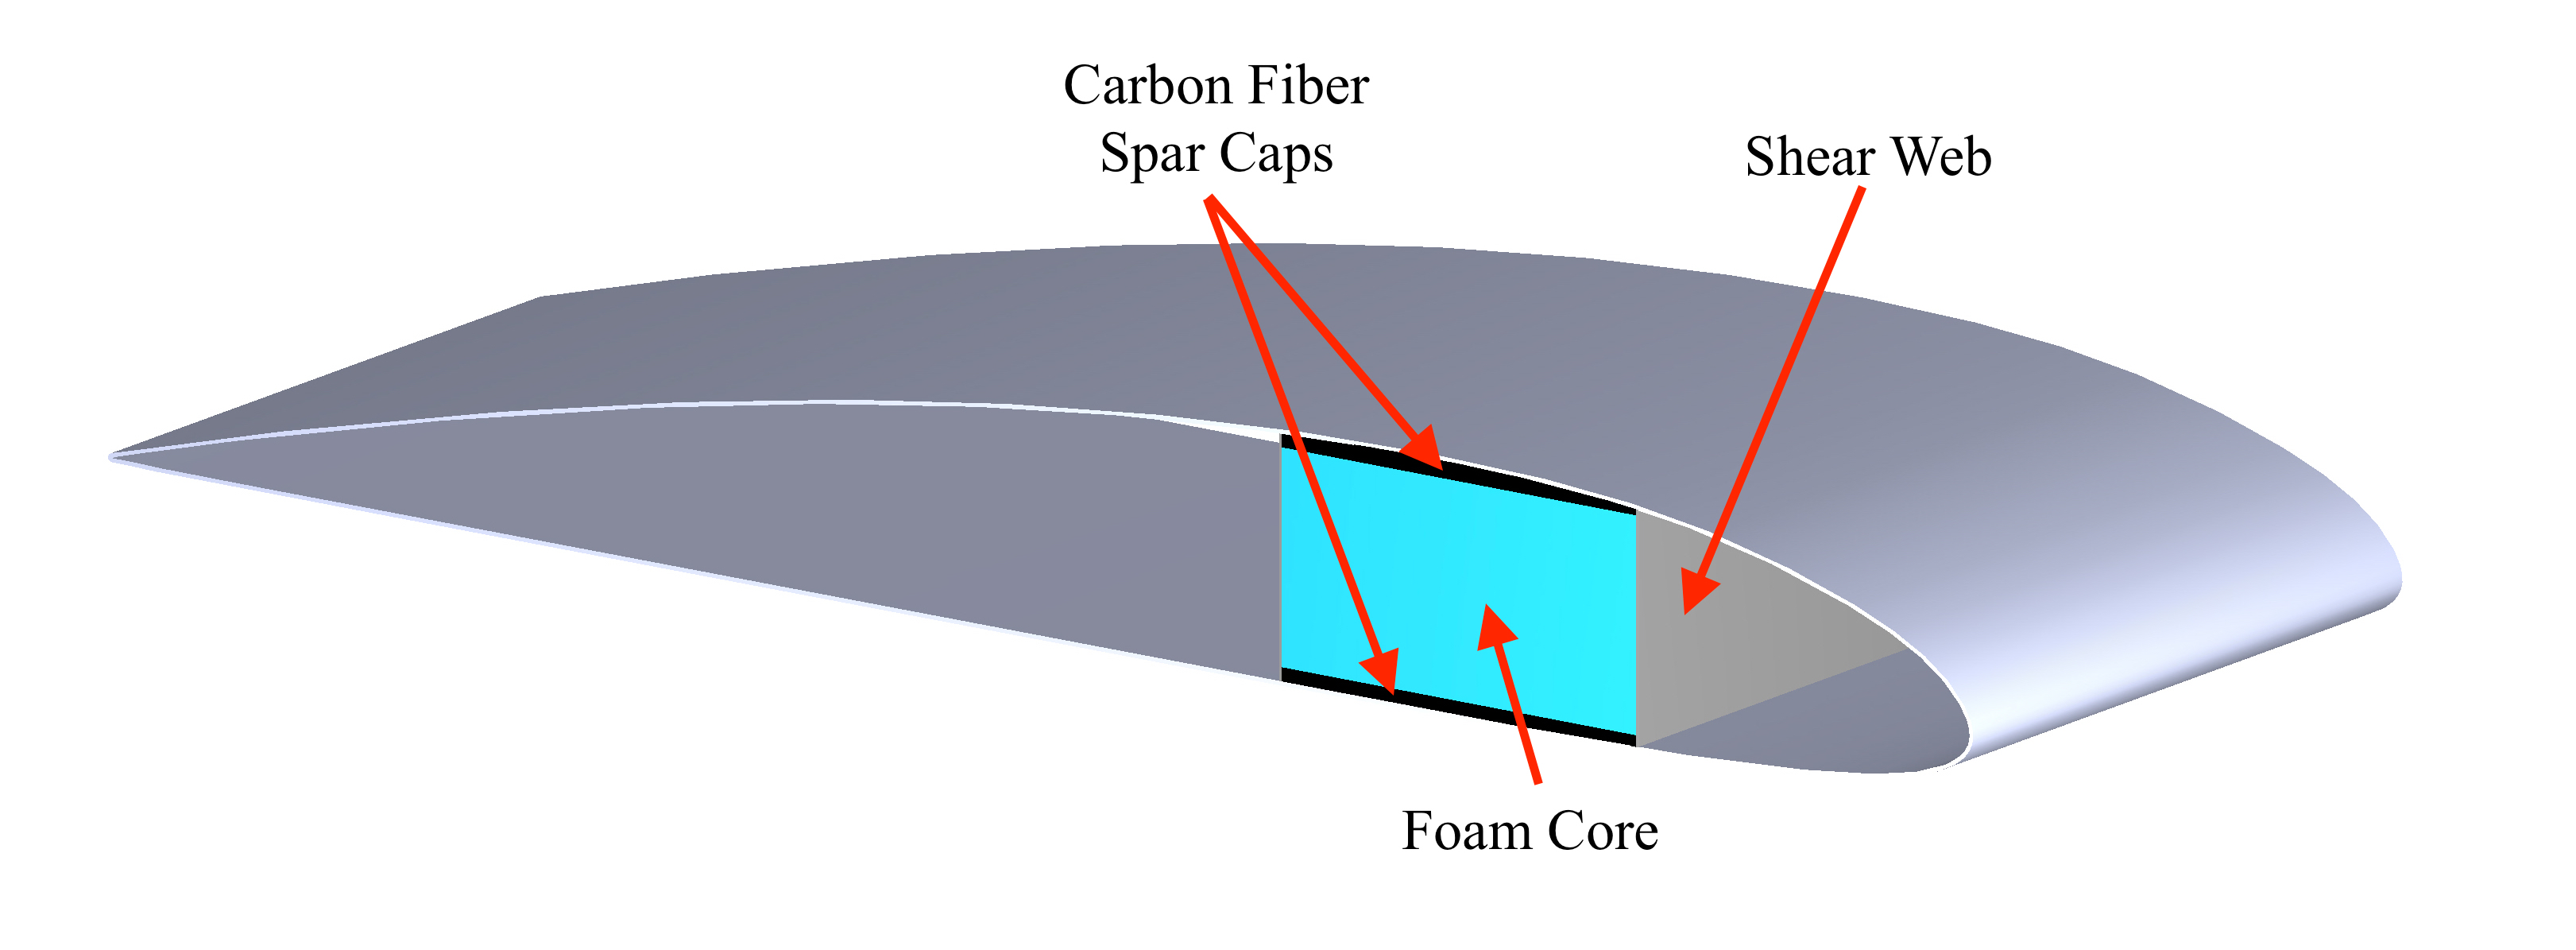
\includegraphics[width=0.8\textwidth,natwidth=3242,natheight=1195]{capspar2.jpg}
    \caption{\textbf{Cross sectional view of a cap spar.}}
	\label{f:capspar}
	\end{center}
\end{figure}

The moment of inertia of the cap spar is modeled by only considering the spar caps, not the foam interior.  
This conservative assumption is made because the contribution of the foam core is much less than that of the spar caps.  
The equation for the moment of inertia\cite{bending} of a cap spar is 

\begin{equation}
    \label{e:moispar}
    I = \frac{w_{\text{cap}}t_{\text{cap}}^3}{6} + 2w_{\text{cap}}t_{\text{cap}}\left( \frac{h_{\text{cap}}}{2} + \frac{t_{\text{cap}}}{2} \right)^2.
\end{equation}

This equation is not GP compatible.  However, using a first order conservative approximation, the moment of inertia can be simplified to be written in a GP-compatible form, 

\begin{equation}
    \label{e:moispar}
    I \leq 2w_{\text{cap}}t_{\text{cap}}\left(\frac{h_{\text{cap}}}{2}\right)^2.
\end{equation}

There are also geometric constraints imposed on the width and thickness.  The total spar cap thickness cannot be greater than the thickness of the airfoil cross section, $\tau_t = 0.115$.  The width of the spar cap is assumed no greater than 30\% of chord, $\tau_w = 0.3$.

\begin{align}
    \label{e:thickness}
    c(y)\tau_t &\geq h_{\text{cap}} + 2t_{\text{cap}} \\
    \label{e:width}
    c(y)\tau_w &\geq w_{\text{cap}} 
    \end{align}

To match the discretized beam model, the spar cross section can also be written in a discretized form such that each section has a unique width and thickness. 

\begin{align}
    I_i &\leq 2w_{\text{cap}_i}t_{\text{cap}_i}\left(\frac{h_{\text{cap}_i}}{2}\right)^2 \\
    c(y)\tau_t &\geq h_{\text{cap}_i} + 2t_{\text{cap}_i} \\
    c(y)\tau_w &\geq w_{\text{cap}_i} 
\end{align}

The wing spar at each section root must be strong enough to withstand the bending moment and stiff enough to not exceed some deflection limit.  Both constraints are imposed in the optimization model as

\begin{align}
    \label{e:stresscont}
    \sigma_{\text{cfrp}} &\geq \mathcal{M}_i \frac{h_{\text{cap}_i}+t_{\text{cap}_i}}{I_i}\\
    \label{e:defcont}
    w_n &\leq w_{\text{max}}.
\end{align}

The ultimate compressive strength for carbon fiber is, $\sigma_{\text{cfrp}} = 570$ [MPa].\cite{carbonfiber}
The tip deflection is constrained to be less than 20\% of the half span, $\frac{w_{\text{max}}}{b/2} = 0.2$.

Finally, the weight of the spar cap is computed as

\begin{align}
    \label{e:sparmass}
    \Delta W_i &\geq \rho_{\text{cfrp}} w_{\text{cap}_i}t_{\text{cap}_i} \frac{b/2}{n-1}g \\
    \label{e:sparmasssum}
    W_{\text{spar}} &\geq 2 \sum\limits_{1}^{n-1} \Delta W_i
\end{align}

where $\rho_{\text{cfrp}} = 1.6$ [g/cm$^3$].\cite{carbonfiber}

\subsection{Wing Skin Weight}

It is assumed that the wing skin is made of carbon fiber.  The weight of the wing skin is 

\begin{equation}
    \label{e:wingskinweight}
    W_{\text{skin}} \geq 2 \rho_{A_{\text{cfrp}}} S g.
\end{equation}

where $\rho_{A_{\text{cfrp}}} = 0.049$ [g/cm$^2$], or approximately the area density of one ply of carbon fiber.\cite{carbonfiber} The wing skin is asssumed not to contribute to the bending stiffness. 

\subsection{Empennage}

An empennage model is added to both the solar-electric and gas powered aircraft models.  The empennage model consists of a single tail boom, horizontal tail and vertical tail.  
The empennage adds both weight and drag to each aircraft.  

The tail boom has a diameter $d$, root wall thickness $t_0$, root moment of inertia $I_0$, modulus $E$, and density $\rho_{\text{cfrp}} = 1.6$ [g/cm$^3$], and length $l_{\text{h}}$. 
The total mass and root bending inertia are imposed in the optimization model as 

\begin{align}
    m &\geq \pi \rho_{\text{cfrp}} t_0 d l_{\text{h}} \left( 1 - \frac{1}{2} k\right) \\
    I_0 &\leq \pi t_0 d^3/8
\end{align}

where the index $k=0$ corresponds to a uniform wall thickness and stiffness, and $k=1$ corresponds to a linear drop-off to zero.  For both the solar-electric and gas powered aircraft $k=0.8$ is assumed.  
When the tail boom is loaded at the endpoint $x=l_{\text{h}}$, by the horizontal tail lift $L_{\text{h}}$, the end deflection angle follows from standard beam analysis

\begin{align}
    \label{e:boomdefl}
    \theta &\geq \frac{L_{\text{h}} l_{\text{h}}^2}{EI_0} \frac{1+k}{2} \\
    L_{\text{h}} &= \frac{1}{2} C_{L_{\text{h}}} \rho V^2 S_{\text{h}}.
\end{align}

The horizontal tail is sized to satisfy a horizontal tail volume coefficient condition, $V_{\text{h}} = 0.45$,\cite{aircraftrules}

\begin{equation}
    V_{\text{h}} = \frac{S_{\text{h}}l_{\text{h}}}{Sc}
\end{equation}

% meet a minimum static margin $\text{SM}_{\text{min}} = 0.35$ and minimum desirable c.g. travel range,
% 
% \begin{equation}
%     \label{e:deltacg}
%     \Delta x_{cg} = (x_{cg})_{\text{aft}} - (x_{cg})_{\text{fwd}} = 0.2
% \end{equation}
% 
% A single constraint, whose derivation is explained in Appendix C, minimizes the horizontal tail volume coefficient $V_{\text{w}}$, while meeting the minimum static margin and minimum c.g. travel range,
% 
% \begin{align}
%     \label{e:smcorr}
%     \text{SM}_{\text{min}} + \frac{\Delta x_{cg}}{c} - \frac{C_{M_{	ext{w}}}}{C_{L_{\text{max}}}} &\leq V_{\text{w}} \mathcal{F}_{NE}^{-1} \frac{m_{\text{h}}}{m_{\text{w}}} \left( 1 - \frac{d\epsilon}{d\alpha}\right) + V_{\text{w}} \frac{-(C_{L_{\text{h}}})_{\text{min}}}{C_{L_{\text{max}}}} \\
%     \label{e:htv}
%     V_{\text{w}} &= \frac{S_{\text{h}}}{S} \frac{l_{\text{h}}}{c}
% \end{align}
% 
% Because this equation is not posynomial, it was reformulated as conservative monomial approximation
% 
% \begin{align}
%     1 &\geq z_{\text{SM}_1} \left(\frac{m_{\text{w}} \mathcal{F}_{NE}}{m_{\text{h}} V_{\text{w}}})\right) + \frac{d\epsilon}{d\alpha} \\
%     z_{\text{SM}_2} &\leq V_{\text{w}}\frac{(C_{L_{\text{h}}})_{\text{min}}}{C_{L_{\text{max}}}} \\
%     \label{e:smcorrmon}
%     z_{\text{SM}_1}^{0.48} z_{\text{SM}_1}^{0.52} &\geq \text{SM}_{\text{min}} + \frac{\Delta x_{cg}}{c} - \frac{C_{M_{	ext{w}}}}{C_{L_{\text{max}}}}
% \end{align}
% 
% where the values, 0.48 and 0.52, are chosen as an approximate percentage that each term is of the right hand side of Equation~\eqref{e:smcorrmon}. 

The vertical tail is sized to meet a conservative tail volume coefficient, $V_{\text{v}}= 0.04$,\cite{aircraftrules}

\begin{equation}
    \label{e:vtv}
    V_{\text{v}} = \frac{S_{\text{v}}}{S} \frac{l_{\text{v}}}{b}
\end{equation}

where $l_{\text{v}}$ is the vertical tail moment arm, assumed to be equal to the horizontal tail moment arm, $l_{\text{v}} = l_{\text{h}}$.

Both the horizontal and vertical tails are assumed to have a carbon fiber skin and solid foam interior where their respective densities are $\rho_{A_{\text{cfrp}}} = 0.049$ [g/cm$^2$], $\rho_{\text{foam}} = 1.5$ [lbf/ft$^3$]. 
The weight of the horizontal and vertical tails is

\begin{align}
    \label{e:htweight}
    W_{\text{h}}/m_{\text{fac}} &= \rho_{\text{foam}} \frac{S_{\text{h}}^2}{b_{\text{h}}} \bar{A} + g\rho_{A_{\text{cfrp}}} S_{\text{h}} \\
    \label{e:vtweight}
    W_{\text{v}}/m_{\text{fac}} &= \rho_{\text{foam}} \frac{S_{\text{v}}^2}{b_{\text{v}}} \bar{A} + g\rho_{A_{\text{cfrp}}} S_{\text{v}}
\end{align}

where $b_{\text{h}}$ and $b_{\text{v}}$ are the spans of the horizontal and vertical tails respectively and $\bar{A}$ is the cross sectional area of the NACA 0008 airfoil. The margin factor $m_{\text{fac}}=1.1$, is included to account for control surfaces, attachment joints, actuators, etc. 

The drag of the empennage was modeled as three separate parts with no interference drag.  The drag of the tail boom is calculated using a turbulent flat plate model,

\begin{align}
    \label{e:boomdrag}
    D_{\text{boom}} &\geq \frac{1}{2} C_f \rho V^2 l_{\text{h}}\pi d \\
    C_f &\geq \frac{0.445}{Re_{\text{boom}}^{0.3}} \\
    Re_{\text{boom}} &= \frac{V\rho l_{\text{h}}}{\mu}
\end{align}

The drag of the horizontal and vertical tails is computed using a GP-compatible fit of XFOIL data for a range of Reynolds numbers and NACA airfoil thicknesses,

\begin{align}
    D_{\text{h}} &\geq \frac{1}{2} c_{d_{\text{h}}} \rho V^2 S_{\text{h}} \\
    D_{\text{v}} &\geq \frac{1}{2} c_{d_{\text{v}}} \rho V^2 S_{\text{v}} \\
    \label{e:taildrag}
    c_{d_{\text{(v,h)}}}^{70.5599} &\geq \num{7.42688d-90} \left( \frac{Re_{\text{(v,h)}}}{\num{1d3}} \right)^{-33.0637}(100 \tau_{\text{(v,h)}})^{18.0419}  \nonumber \\
                 & + \num{5.02826d-163}\left(\frac{Re_{\text{(v,h)}}}{\num{1d3}}\right)^{-18.7959} (100\tau_{\text{(v,h)}})^{53.1879} \\
                 &+ \num{4.22901d-77}\left(\frac{Re_{\text{(v,h)}}}{\num{1d3}}\right)^{-41.1704} (100\tau_{\text{(v,h)}})^{28.4609} \nonumber \\
    Re_{\text{v}} &= \frac{V\rho S_{\text{v}}/b_{\text{v}}}{\mu} \\
    Re_{\text{h}} &= \frac{V\rho S_{\text{h}}/b_{\text{h}}}{\mu} 
\end{align}

where the selected airfoil is the NACA 0008 for both the horizontal and vertical tails (i.e. $\tau_{\text{(v,h)}} = 0.08$). 
The XFOIL data was generated for a zero angle of attack, based upon steady level flight where neither surface is generating lift.  
A comparison of the XFOIL data and Equation~\eqref{e:taildrag} is shown in Figure~\ref{f:taildragpolar}.

\begin{figure}[H]
	\begin{center}
	\includegraphics[width=0.6\textwidth,natwidth=538,natheight=405]{taildragpolar.pdf}
    \caption{\textbf{Posynomial fit (solid lines) to XFOIL data (circles). (Log-space RMS error = 0.0173)}}
	\label{f:taildragpolar}
	\end{center}
\end{figure}

\subsection{Elliptcal Fuselage for Gas Powered Aircraft}

For the gas powered aircraft it is assumed that the fuel is carried in an elliptically shaped fuselage.  The fuselage will increase the overall weight and drag of the aircraft.  The solar-electric powered aircraft is assumed to carry the batteries in the wings will therefore have a small fuselage whose effects will be ignored.  

The driving constraint for the size of the fuselage is to ensure that all of the fuel required for the mission can fit inside the fuselage, 

\begin{equation}
    \label{e:fusevol}
    \mathcal{V}_{\text{fuse}} \geq \frac{W_\text{fuel}}{\rho_\text{fuel}}
\end{equation}

where the fuel is assumed to have a density $\rho_\text{fuel} = 6.01$ [lbf/gallon].  The dimensions of the fuselage are constrained by

\begin{equation}
    \label{e:fusevol2}
    \mathcal{V}_{\text{fuse}} \leq \frac{4}{3}\pi \frac{l_{\text{fuse}}}{2}R_{\text{fuse}}^2
\end{equation}

where $l_{\text{fuse}}$ is the length of the fuselage and $R_{\text{fuse}}$ is the radius. Using the length and radius, the surface area can be calculated using Thomsen's approximation,\cite{ellipsoidSA}

\begin{equation}
    \label{e:fusesa}
    3 \left( \frac{S_{\text{fuse}}}{\pi} \right)^{1.6075} \geq 2(2l_{\text{fuse}}R_{\text{fuse}})^{1.6075} + (4R_{\text{fuse}}^2)^{1.6075}.
\end{equation}

The weight of the fuselage is constrained by

\begin{equation}
    \label{e:fuseweight}
    W_{\text{fuse}} \geq S_{\text{fuse}} \rho_{A_{\text{cfrp}}} g
\end{equation} 

where $\rho_{A_{\text{cfrp}}} = 0.0975$ [g/cm$^2$], or the area density of two plys of carbon fiber.\cite{carbonfiber}  The surface area is also used to calculate the drag assuming a skin friction based drag model,

\begin{align}
    \label{e:fusedrag}
    D_{\text{fuse}} &\geq C_f k_{\text{fuse}} \frac{1}{2} \rho V^2 S_{\text{fuse}} \\
    C_f &\geq \frac{0.455}{Re^{0.3}}
\end{align}

where $k_{\text{fuse}}$ is the form factor approximated by\cite{raymer}

\begin{equation}
    \label{e:fuseform}
    k_{\text{fuse}} \geq 1 + \frac{60}{(l_{\text{fuse}}/2R_{\text{fuse}})^3} + \frac{(l_{\text{fuse}}/2R_{\text{fuse}})}{400}.
\end{equation}

\subsection{Engine Weight}

The solar-electric powered aircraft has a motor whose weight is based on the approximation\cite{electricengine}

\begin{equation}
    \label{e:electricengine}
    P_{\text{max}} = B_{PM} m_{\text{motor}}
\end{equation}

where $m_{\text{motor}}$ is the motor mass, $P_{\text{max}} \geq P_{\text{oper}}$ is the maximum operating power, and the power to mass ratio is $B_{PM} = 4140.8$ [W/kg]. \\

The engine weight of the gas powered aircraft is governed by a simple power law derived from existing two-stroke and four-stroke engines\cite{gasengine}

\begin{equation}
    \label{e:powerlaw}
    \frac{W_{\text{engine}}}{W_{\text{engine-ref}}} = 1.27847 \left(\frac{P_{\text{SL-max}}}{P_{\text{ref}}} \right)^{0.772392}
\end{equation}

where $W_{\text{engine-ref}} = 10$ [lbs] and $P_{\text{ref}} = 10$ [hp].  Equation~\eqref{e:powerlaw} was found using techniques described in Hoburg et. al\cite{fitting}. Equation~\eqref{e:powerlaw} is compared to the data in Figure~\ref{f:powervsweightfit}.

\begin{figure}[H]
	\begin{center}
	\includegraphics[width=0.6\textwidth,natwidth=524,natheight=405]{powervsweightfit.pdf}
    \caption{\textbf{Power law fit to University of North Dakota engine weight data\cite{gasengine}. (Log-space RMS error = 0.34)}}
	\label{f:powervsweightfit}
	\end{center}
\end{figure}

\subsection{Gas Powered Engine Performance}

Two characteristics of gas engines affect the performance of long-endurance aircraft.  
The first is brake specific fuel consumption, $\text{BSFC}$; a lower $\text{BSFC}$ will result in increased endurance.  
The second is the lapse rate.  
Assuming a propeller driven aircraft and a naturally aspirated engine, as the aircraft reaches higher altitudes, the engine will have decreased available power. 
To account for these two affects a two-stroke, double cylinder engine, the DF70 from RCV Engines Ltd, England, was selected as a representative engine.  
RCV Engines Ltd provided manufacturing data that was used to generate representative performance curves.\cite{rcvengines}
It is assumed that engines of a similar size will perform similarly to the DF70 engine.  
This engine performance model is only valid for internal combustion engines.

\subsubsection{Brake Specific Fuel Consumption Constraint}

To capture throttling effects as aircraft weight decreases, a GP-compatible curve was generated from the DF70 data to relate $\text{BSFC}$ and shaft power, 

\begin{equation}
    \label{e:rpmtobsfc}
    \left( \frac{\text{BSFC}}{\text{BSFC}_{100\%}} \right)^{18.5563} \geq \num{8.66321d-3}\left( \frac{P_{\text{shaft}}}{P_{\text{max}}}\right)^{-7.70161} + 1.38628\left( \frac{P_{\text{shaft}}}{P_{\text{max}}} \right)^{1.12921} \\
\end{equation}

where $\text{BSFC}_{100\%} = 0.3162$ [kg/kW/hr].\cite{rcvengines}
Using this approximation the required shaft power determines the $\text{BSFC}$.
A comparison of the GP-compatible approximation to the manufacturing data from RCV engines is presented in Figure~\ref{f:powervsweightfit}. A comparison of the DF70 data provided by RCV Engine Ltd in Figure~\ref{f:powervsweightfit} to the $\text{BSFC}$ to power curves in Goering\cite{bsfcperf} verify that this performance curve is representative of engines of similar sizes. 

\begin{figure}[H]
	\begin{center}
	\includegraphics[width=0.6\textwidth,natwidth=530,natheight=414]{powertobsfcfit.pdf}
    \caption{\textbf{Representative engine performance fit based on RCV Engine Ltd data.  (Log-space RMS error = 0.007) }}
	\label{f:powervsweightfit}
	\end{center}
\end{figure}

\subsubsection{Engine Lapse Rate Calculation}

The lapse rate $L_{\text{eng}}(h) \leq 1$, is assumed to affect the maximum power output,

\begin{equation}
    \label{e:lapse}
    L_{\text{eng}}(h) \equiv \frac{P_{\text{max}}}{P_{\text{SL-max}}}.
\end{equation}

The lapse is calculated from the required flight altitude $h=15,000$ [ft], prior to the optimization solve using an approximate engine loss rate for normally aspirated engines of 3.5\% hp per 1000 ft,\cite{enginelapse}

\begin{equation}
    \label{e:lapsefit}
    L_{\text{eng}}(h) = 1 - \frac{0.035}{1000 \text{ [ft]}} h.
\end{equation}

\subsection{Climb Constraints}

Because the gas engine is naturally aspirated, as the aircraft climbs there will be less available power.  
The climb constraint ultimately sizes the engine because at the top of climb, when the least amount of power is available, the engine must provide the necessary power to meet a minimum climb rate, 

\begin{equation}
    \label{e:climbrate}
    \dot{h} \geq 100 \text{ [ft/min]}.
\end{equation}

The climb rate affects the required thrust, and therefore the required power during climb, 

\begin{equation}
    \label{e:climb}
    T \geq \frac{1}{2} C_D \rho V^2 S + W \frac{\dot{h}}{V}
\end{equation}

where $W$ is the weight of the aircraft during climb.  

\subsection{Weight Breakdown}

The weight of each component of both the gas and solar platforms is summed to constrain the max take off weight.  
The structural weight comprises the weight of the wing, fuselage, horizontal and vertical stabilizers, and engine. 
The weight breakdown for the gas powered aircraft is a summation of the structural weight, the total fuel weight, and the payload weight. 

\begin{align}
    \label{e:weightmtow}
    \text{MTOW} &\geq W_{\text{structural}}  + W_{\text{payload}} + W_{\text{fuel}} + W_{\text{engine}} \\
    W_{\text{structural}} &\geq W_{\text{wing}} + W_{\text{boom}} + W_{\text{h}}+ W_{\text{v}} + W_{\text{fuse}}
\end{align}

A similar weight breakdown is done for the solar-electric powered aircraft, 

\begin{align}
    \label{e:weightsmtow}
    \text{MTOW} &\geq W_{\text{structural}} + W_{\text{payload}} + W_{\text{solar}} + W_{\text{batt}} + W_{\text{motor}} \\
    W_{\text{structural}} &\geq W_{\text{wing}} + W_{\text{boom}} + W_{\text{h}}+ W_{\text{v}} \\
    W_{\text{solar}} &\geq \rho_{\text{solar}} S_{\text{solar}} g \\
    W_{\text{batt}} &\geq \frac{E_{\text{batt}}}{h_{\text{batt}}} g
\end{align}

where the solar cell density is $\rho_{\text{solar}} = 0.27$ [kg/m$^2$].\cite{solartech}\cite{solarparam}
Lithim-sulfur batteries are selected with a battery specific energy $h_{\text{batt}} = 350$ [Whr/kg].\cite{lithiumsul}
The payload weight is assumed to be $W_{\text{payload}} = 10$ [lbs].

\section{Results}

To compare the gas-powered and solar-electric architectures the optimization models were solved by minimizing the max take off weight across different bands of latitudes. Figure~\ref{f:latvsmtowtrade} shows this trade study evaluated at the 80th, 90th and 95th percentile wind speeds.  
Each point on the graph is a unique solution to the optimization model for the stated assumptions and constants.
The gas powered optimization model contains 606 free variables and the solar-electric powered optmization model contains between 165 and 585 free variables depending on latitude band requirement. 

\begin{figure}[H]
	\begin{center}
	\includegraphics[width=0.6\textwidth,natwidth=528,natheight=405]{mtowvslat.pdf}
    \caption{\textbf{Gas archicture feasible for all latitudes. Next integer latitude for each solar-electric curve is infeasible.}}
    \label{f:latvsmtowtrade}
	\end{center}
\end{figure}

One way to interpret Figure~\ref{f:latvsmtowtrade} is that a solar-powered aircraft weighing 190 lbs is able to operate between $\pm$30 degrees North latitude in 90th percentile wind speeds.  
This analysis shows that gas powered architectures are able to operate in more locations than solar-electric powered aircraft.  
The gas powered aircraft curves level off around 38 degrees latitude because wind speeds are highest at that latitude at 15,000 ft. 
Thus, if the gas powered aircraft can fly at 38 degrees latitude it can fly in any band of latitudes.  
On the other hand, solar-electric powered aircraft design becomes infeasible at higher latitudes because even though wind speeds peak around 42 degrees latitude at 60,000 ft, the combination of lower solar flux and higher wind speeds makes it difficult to reach latitude bands greater than $\pm$30 degrees. 

Because gas-powered aircraft are endurance limited by the amount of fuel that they can carry, a trade study was done for the gas powered aircraft to determine how weight increases for longer endurance.
Figure~\ref{f:spanvsendurance} shows the endurance versus size analysis for a gas powered aircraft by minimizing max take off weight for an aircraft capable of flying at any latitude. 

\begin{figure}[H]
	\begin{center}
	\includegraphics[width=0.6\textwidth,natwidth=527,natheight=405]{mtowvsendurance.pdf}
    \caption{\textbf{Endurance and size trade study for gas powered architecture.}}
	\label{f:spanvsendurance}
	\end{center}
\end{figure}

Changing the objective function can be informative to the design space. 
High efficiency solar cells are expensive and from a manufacturing perspective, a larger aircraft that requires fewer solar cells could be advantageous.
By altering the objective function to solar cell area it is observed that when the objective function is solar cell area the airplane is slightly bigger but requires fewer solar cells. (Figure~\ref{f:solarobjcomp})

\begin{figure}[H]
 \begin{subfigmatrix}{2}% number of columns
     \subfigure[Wingspan\label{f:span}]{\includegraphics[natwidth=511,natheight=398]{solarobjcomp.pdf}}
     \subfigure[Solar Cell Area\label{f:solarcell}]{\includegraphics[natwidth=514,natheight=405]{solarobjcomp2.pdf}}
 \end{subfigmatrix}
    \caption{\textbf{Solar aircraft sizing study for two different objective functions: wing span $b$, and solar cell area $S_{\text{solar}}$.}}
    \label{f:solarobjcomp}
\end{figure}

\subsection{Changing Assumptions}

By altering the aircraft structural model it can be observed how air density trades for wing weight. 
It might be assumed that because the wind speeds are lowest at 67,000 ft at 29 degrees latitude, that the aircraft will always fly at 67,000 ft.  
If it is assumed that the structural weight of the aircraft can be modeled as a fraction of the total weight 

\begin{equation}
    W_{\text{structural}} \geq \text{MTOW} f_{\text{structural}}
\end{equation}

where $f_{\text{structural}} = 0.35$, then the optimized flight altitude is almost exactly 67,000 ft as shown in Figure~\ref{f:altoper}.  
However, if the structural weight is represented by the more detailed model as explained in Section IV, larger wings have a weight penalty and the optimization trades air density for wing weight.
Therefore, by adding a structural model the optimization seeks a smaller wing to save weight and operates at a lower altitude to increase density. 

\begin{figure}[H]
	\begin{center}
	\includegraphics[width=0.6\textwidth,natwidth=519,natheight=405]{windaltoper.pdf}
 \caption{\textbf{Comparison of simplified and detailed structural models highlights trade between wing weight and air density.}}
 \label{f:altoper}
	\end{center}
\end{figure}

Another interesting result is the operating lift to drag ratio for the gas powered aircraft.  
The optimum lift to drag ratio to maximize endurance for gas powered aircraft is at the maximum $C_L^{1.5}/C_D$.\cite{br2}  
However, while station keeping, the aircraft will maintain a constant velocity during high wind speeds.  
At a constant velocity or constant Reynolds number the lift to drag ratio will not be at the maximum $C_L^{1.5}/C_D$.  
If it is assumed that wind speeds are negligible or that station-keeping is not important then velocity will be optimized such that the lift to drag ratio is at the maximum $C_L^{1.5}/C_D$ as shown in Figure~\ref{f:polarmission}.

\begin{figure}[H]
	\begin{center}
	\includegraphics[width=0.6\textwidth,natwidth=555,natheight=415]{polarmission.pdf}
    \caption{\textbf{Wind speed constraint moves lift to drag ratio off maximum $(C_L^{1.5}/C_D)$ point (plus signs). Solid lines are drag polars.}}
 \label{f:polarmission}
	\end{center}
\end{figure}

The solar aircraft size and design depends on the assumed solar cell efficiency and battery specific energy. 
By solving the model for different assumed solar cell efficiency and battery specific energy values a broader picture of the design space is achieved.   
Figure~\ref{f:solarcontours} shows a matrix contour map of the solar-electric powered aircraft for multiple solar cell efficiencies, battery energy densities, latitudes, and percentile wind speeds.
Each point in Figure~\ref{f:solarcontours} is a unique design for minimum wing span. 
The infeasible regions and contour shapes would change for different assumed constant values. 

 \begin{figure}[H]
 \begin{subfigmatrix}{3}% number of columns
  \subfigure[35th Latitude, 80\% Wind Speed]{\includegraphics[natwidth=542,natheight=414]{bcontourl35a80.pdf}}
  \subfigure[35th Latitude, 85\% Wind Speed]{\includegraphics[natwidth=542,natheight=414]{bcontourl35a85.pdf}}
  \subfigure[35th Latitude, 90\% Wind Speed]{\includegraphics[natwidth=542,natheight=414]{bcontourl35a90.pdf}}
  \subfigure[30th Latitude, 80\% Wind Speed]{\includegraphics[natwidth=542,natheight=414]{bcontourl30a80.pdf}}
  \subfigure[30th Latitude, 85\% Wind Speed]{\includegraphics[natwidth=542,natheight=414]{bcontourl30a85.pdf}}
  \subfigure[30th Latitude, 90\% Wind Speed]{\includegraphics[natwidth=542,natheight=414]{bcontourl30a90.pdf}}
  \subfigure[25th Latitude, 80\% Wind Speed]{\includegraphics[natwidth=542,natheight=414]{bcontourl25a80.pdf}}
  \subfigure[25th Latitude, 85\% Wind Speed]{\includegraphics[natwidth=542,natheight=414]{bcontourl25a85.pdf}}
  \subfigure[25th Latitude, 90\% Wind Speed]{\includegraphics[natwidth=542,natheight=414]{bcontourl25a90.pdf}}
 \end{subfigmatrix}
 \caption{\textbf{Maxtrix of minimum wing span solar-electric aircraft designs. Values of assumed constants are given throughout the text.}}
 \label{f:solarcontours}
\end{figure}

\subsection{Sensitivities}

When a GP is solved, the sensitivity of the optimal objective value with respect to each constraint is also returned.  
From this information, the sensitivity of the optimal objective value to each fixed variable can be extracted.\cite{hoburgthesis} 
While sensitivities are local and therefore only exact for small changes, they provide useful information about the relative importance of various design variables. 
For example, if the objective function were MTOW and the sensitivity to battery specific energy were 0.5, then a 1\% increase in the solar cell efficiency would result in a 0.5\% increase in weight.  
Tables~\ref{t:sens} and~\ref{t:gassens} show the variables with the highest sensitivities for the solar-electric and gas powered architectures respectively, where the objective was max take off weight.

For the solar-electric aircraft, it is interesting to note that the battery discharge efficiency sensitivity is higher than the battery charge efficiency sensitivity.
This occurs because the discharge efficiency directly affects the required battery size, whereas the charge efficiency only does so indirectly. 

Sensitivities can also be used to give insight into the break-even point (in terms of cost) for investing in various technologies.  
For example, both batteries and solar cells are expensive and important to the design.  
The sensitivity to the battery specific energy is -2.27 and the sensitivity to solar cell efficiency is -1.29 for the 25th latitude and 85th percentile winds. 
The ratio of their magnitudes is 1.76.  
Therefore, the break-even point for investing in these technologies occurs when a given percentage improvement in battery specific energy costs 1.76 times as much to achieve as the same percentage improvement in solar cell efficiency. 

\input{sens.generated.tex}

\input{gassens.generated.tex}

\section{Conclusion}

Using geometric programming as a means of evaluation of the design space, high level intuition and understanding about design trade studies for long-endurance aircraft and their driving requirements is achieved.  
One high level discovery is the importance of wind speed.  
If station keeping during any season or latitude is critical to the mission of a proposed aircraft, then that requirement is more likely to be met by a gas-powered architecture.
However, if that constraint can be relaxed such that the aircraft only needs to station keep for 80\% of the time, then for certain latitudes, a solar powered aircraft could achieve greater endurance.
An unsurprising discovery is the sensitivity of the solar-powered aircraft to the battery specific energy and solar cell efficiency.  Using higher energy density batteries can result in significant weight and performance savings.  
The rapid solve time of geometric programming is able to present these trade studies and give intuition into design trades by quantifying the disparity in performance between the two options.


% produces the bibliography section when processed by BibTeX
\bibliography{biblibrary}
\bibliographystyle{aiaa}

\section*{Appendix A}

\subsection{Wind Speed Constraints}

The each wind speed constraint follows the following form

\begin{equation}
    \label{e:windspeedgen}
    \left(\frac{V_{\text{wind}}}{V_{\text{ref}}}\right)^{\alpha} \geq c_1 \rho^{e_{1,1}}p_{\text{wind}}^{e_{1,2}} + c_2 \rho^{e_{2,1}}p_{\text{wind}}^{e_{2,2}} + c_3 \rho^{e_{3,1}}p_{\text{wind}}^{e_{3,2}} + c_4 \rho^{e_{4,1}}p_{\text{wind}}^{e_{4,2}}
\end{equation}

Table~\ref{t:windvals} lists the values of the coefficients and exponents of Equation~\eqref{e:windspeedgen} for latitudes 20-60. Each generated constraint has a RMS error of less than 5\% valid for altitude ranges between 48,000 and 80,000 ft. 

\tiny
\begin{longtable}{lccccccccccccc} \\
\label{t:windvals} \\
    \caption{Wind Speed Function Coefficients and Exponents} \\
    \toprule
    \toprule
    Latitude & $c_1$ & $e_{1,1}$ & $e_{1,2}$ & $c_2$ & $e_{2,1}$ & $e_{2,2}$ & $c_3$ & $e_{3,1}$ & $e_{3,2}$ & $c_4$ & $e_{4,1}$ & $e_{4,2}$ & $\alpha$ \\
    \midrule
20 & 9.77e-15 & -8.45 & 53.1 & 5.26e+04 & 9.98 & 6.26 & 1.97e+03 & 7.66 & 39.3 & 3.9e-14 & -7.26 & 10.6 & 5.53\\
21 & 1.01e-13 & -7.88 & 47.9 & 6.66e-13 & -6.62 & 9.18 & 8.09e+04 & 9.61 & 5.48 & 1.36e+03 & 7.04 & 35.8 & 5.03\\
22 & 1.12e+05 & 9.65 & 5.29 & 1.53e-13 & -7.75 & 47.6 & 7.58e-13 & -6.64 & 8.9 & 2.03e+03 & 7.11 & 35 & 5.06\\
23 & 2.68e+03 & 7.11 & 34 & 1.07e-12 & -6.61 & 8.67 & 1.35e+05 & 9.6 & 5.09 & 4.2e-13 & -7.46 & 48.6 & 5.08\\
24 & 4.81e+03 & 7.4 & 33.6 & 6.8e-13 & -7.25 & 48.3 & 1.95e+05 & 9.81 & 5.08 & 4.84e-13 & -6.87 & 8.91 & 5.31\\
25 & 2.14e-12 & -6.86 & 48 & 6.28e+03 & 7.5 & 33.3 & 2.02e+05 & 9.8 & 5.12 & 3.1e-13 & -7.06 & 9.17 & 5.48\\
26 & 7.48e+03 & 7.51 & 34.7 & 2.95e+05 & 9.9 & 5.26 & 3.13e-13 & -7.14 & 9.52 & 7.03e-12 & -6.51 & 51.4 & 5.59\\
27 & 3.62e+05 & 10 & 5.44 & 7.09e-12 & -6.54 & 51.1 & 1.29e-13 & -7.44 & 9.71 & 8.93e+03 & 7.57 & 36.3 & 5.82\\
28 & 7.9e-14 & -7.65 & 9.68 & 8.89e+03 & 7.5 & 36.9 & 3.28e+05 & 9.95 & 5.58 & 6.85e-12 & -6.64 & 49.3 & 5.96\\
29 & 6.97e-14 & -7.79 & 9.85 & 2.3e+05 & 9.71 & 5.72 & 7.67e+03 & 7.34 & 36.4 & 1.15e-11 & -6.58 & 50.3 & 6.02\\
30 & 4.2e-14 & -8.05 & 10.2 & 1.29e+05 & 9.38 & 6 & 5.8e+03 & 7.15 & 36.4 & 1.44e-11 & -6.62 & 52.2 & 6.12\\
31 & 2.17e-12 & -7.2 & 57.6 & 9.1e+03 & 7.56 & 40.5 & 1.22e-15 & -9.09 & 11.8 & 1.26e+05 & 9.68 & 7.21 & 6.89\\
32 & 6.21e+04 & 9.3 & 7.9 & 3.54e-12 & -7.12 & 58.1 & 5.23e-16 & -9.45 & 12.2 & 6e+03 & 7.32 & 42.5 & 7.07\\
33 & 1.86e-16 & -9.86 & 12.8 & 2.81e+04 & 8.91 & 8.68 & 3.98e+03 & 7.13 & 44.5 & 8.01e-12 & -6.89 & 58.7 & 7.28\\
34 & 9.95e+03 & 8.43 & 9.54 & 4.7e-17 & -10.4 & 13.5 & 2.66e+03 & 6.97 & 46.7 & 1.19e-11 & -6.79 & 61 & 7.55\\
35 & 2.92e+03 & 7.59 & 9.37 & 1.58e-10 & -6.07 & 60.4 & 4.05e-16 & -9.88 & 13.2 & 1.05e+03 & 6.33 & 46.2 & 7.21\\
36 & 456 & 5.77 & 45 & 3.4e-15 & -9.35 & 12.8 & 834 & 6.79 & 8.98 & 1.23e-09 & -5.52 & 58.8 & 6.92\\
37 & 5.15e-14 & -8.63 & 12.1 & 225 & 5.94 & 8.34 & 8.45e-09 & -5.03 & 57.5 & 196 & 5.19 & 43.2 & 6.52\\
38 & 84.8 & 4.63 & 41.6 & 4.69e-08 & -4.61 & 55.3 & 67.8 & 5.13 & 7.68 & 8.55e-13 & -7.87 & 11.2 & 6.1\\
39 & 1.65e-11 & -7.05 & 10.1 & 35.7 & 4.06 & 40.1 & 22.4 & 4.33 & 6.95 & 2.55e-07 & -4.18 & 51.7 & 5.6\\
40 & 16.7 & 3.57 & 38.4 & 2.62e-10 & -6.28 & 9.05 & 1.32e-06 & -3.75 & 48 & 8.73 & 3.63 & 6.25 & 5.11\\
41 & 3.42e-09 & -5.56 & 7.84 & 3.93 & 2.99 & 5.53 & 8.86e-06 & -3.19 & 43.4 & 11.2 & 3.27 & 37.3 & 4.6\\
42 & 2.06 & 2.42 & 4.8 & 4.04e-08 & -4.87 & 6.63 & 10.3 & 3.16 & 35.8 & 6.03e-05 & -2.61 & 39.2 & 4.07\\
43 & 13.8 & 3.32 & 34.9 & 0.000428 & -2.01 & 36.7 & 1.27 & 1.93 & 4.09 & 4.21e-07 & -4.22 & 5.58 & 3.55\\
44 & 0.929 & 1.54 & 3.39 & 19.9 & 3.54 & 34.2 & 3.77e-06 & -3.6 & 4.62 & 0.00191 & -1.54 & 34.3 & 3.03\\
45 & 0.0061 & -1.16 & 32.6 & 2.75e-05 & -3.04 & 3.83 & 0.783 & 1.24 & 2.76 & 27.5 & 3.75 & 34.2 & 2.55\\
46 & 35.2 & 3.97 & 32.9 & 0.000197 & -2.47 & 3.02 & 0.758 & 1.01 & 2.13 & 0.0176 & -0.791 & 30.5 & 2.04\\
47 & 0.00143 & -1.89 & 2.2 & 42.2 & 4.28 & 28.5 & 0.816 & 0.811 & 1.47 & 0.046 & -0.43 & 28.9 & 1.49\\
48 & 0.926 & 0.622 & 0.814 & 0.0108 & -1.29 & 1.34 & 0.106 & -0.0538 & 28.2 & 57.2 & 4.99 & 20 & 0.895\\
49 & 56.5 & 5.67 & 11.3 & 0.128 & 0.183 & 27.4 & 0.95 & 0.455 & 0.349 & 0.0533 & -0.793 & 0.695 & 0.445\\
50 & 0.869 & 0.355 & 0.148 & 24.1 & 5.47 & 7.62 & 0.0838 & 0.217 & 27.1 & 0.139 & -0.487 & 0.358 & 0.229\\
51 & 4.88 & 4.99 & 5.72 & 0.657 & 0.238 & 0.0196 & 0.0293 & 0.214 & 27.7 & 0.345 & -0.21 & 0.116 & 0.0703\\
52 & 0.00842 & 0.166 & 28 & 0.834 & 4.31 & 4.86 & 0.615 & -0.0754 & 0.0355 & 0.383 & 0.186 & -0.0168 & 0.0212\\
53 & 0.307 & 0.168 & -0.0266 & 0.335 & 3.6 & 4.1 & 0.687 & -0.0538 & 0.0264 & 0.00564 & 0.12 & 27.7 & 0.0155\\
54 & 0.00497 & 0.0916 & 27.5 & 0.223 & 3.09 & 3.42 & 0.54 & -0.067 & 0.0346 & 0.449 & 0.0992 & -0.0245 & 0.0144\\
55 & 0.429 & -0.0809 & 0.0543 & 0.00527 & 0.0771 & 27.7 & 0.206 & 2.77 & 3.25 & 0.553 & 0.0722 & -0.0305 & 0.0158\\
56 & 0.134 & 2.62 & 3.28 & 0.628 & 0.0434 & -0.0319 & 0.00348 & 0.0804 & 28 & 0.358 & -0.072 & 0.0644 & 0.0106\\
57 & 0.00421 & 0.0943 & 28 & 0.0734 & -0.168 & 0.207 & 0.905 & 0.0123 & -0.013 & 0.155 & 2.47 & 3.06 & 0.0128\\
58 & 0.00709 & 0.107 & 28.8 & 0.0366 & -0.258 & 0.474 & 0.253 & 2.33 & 2.98 & 0.921 & 0.00373 & -0.013 & 0.0225\\
59 & 0.0242 & 0.892 & 28.4 & 0.000155 & -1.21 & 16.1 & 0.945 & -0.0147 & 0.0161 & 0.188 & 1.98 & 1.32 & 0.0233\\
60 & 0.0173 & 0.691 & 28.1 & 0.948 & -0.0136 & 0.015 & 0.209 & 2.15 & 1.6 & 7.54e-05 & -1.41 & 14.3 & 0.0222 \\
\bottomrule
\end{longtable}
\normalsize

\section*{Appendix B}

\subsection{Discussion on the use of the \emph{JH01} airfoil}

The \emph{sd7032} airfoil was redesigned to prevent drag creep by weakening the pressure spike associated with premature separation at higher Reynolds numbers.  
Figure~\ref{f:jhcps} shows the pressure distributions generated in XFOIL of the \emph{JH01} airfoil at $C_L=0.0$ and $C_L=1.35$ with $Re=\num{3d5}$.
The redesigned airfoil was named \emph{JH01}. We would like to thank Mark Drela for the redesign.

\begin{figure}[H]
 \begin{subfigmatrix}{2}% number of columns
     \subfigure[$C_L=0.0$\label{f:cpmin}]{\includegraphics[width=0.35\textwidth,natwidth=612,natheight=792,angle=-90]{cpmin.pdf}}
     \subfigure[$C_L=1.35$\label{f:cpmax}]{\includegraphics[width=0.35\textwidth,natwidth=612,natheight=792,angle=-90]{cpmax.pdf}}
 \end{subfigmatrix}
 \caption{\textbf{Pressure coefficient plots at the minimum and maximum expected $C_L$ at Reynolds number $Re=\num{3d5}$.}}
 \label{f:jhcps}
\end{figure}

% \section*{Appendix C}
% 
% To derivation of Equation~\eqref{e:smcorr} begins with the moment about the aircraft's center of mass
% 
% \begin{align}
%     \label{e:mcenter}
%     M_{cg} &= M_{\text{w}} + (x_{cg} - x_{ac})L_{\text{w}} - l_{\text{h}} L_{\text{h}} \\
%     \label{e:eq6}
%     \frac{M_{cg}}{qSc} = C_m &= C_{m_{\text{w}}} + \frac{x_{cg} - x_{ac}}{c} C_{L_W} - V_{\text{w}} C_{L_{\text{h}}}
% \end{align}
% 
% It is assumed that the tail boom's effective root location is at the wing's aerodynamic center $x_{ac}$, and that the tail's pitching moment about its own aerodynamic center is negligible. 
% 
% Using moment and lift approximations
% 
% \begin{align}
%     C_{m_{\text{w}}} &= constant \\
%     C_{L_W} &= C_{L_{W_0}} + m_{\text{w}} \alpha \\
%     \label{e:eq10}
%     C_{L_{\text{h}}} &= C_{L_{h_0}} + m_{\text{h}} \left[\left( 1 - \frac{d\epsilon}{d\alpha}\right) - \theta \right] + C_{L_{h_{\delta}}}\delta_e \\
%     m_{\text{w}} &= \frac{2\pi}{1 + 2/AR_{\text{w}}} \\
%     m_{\text{h}} &= \frac{2\pi}{1 + 2/AR_{\text{h}}}
% \end{align}
% 
% where $\epsilon$ is the wing's downwash angle seen at the tail. Using a vortex approximation and neglecting taper effects, we can estimate
% 
% \begin{equation}
%     \frac{d\epsilon}{d\alpha} = \frac{m_{\text{w}}}{4\pi} \frac{c}{l_{\text{h}}}
% \end{equation}
% 
% so that \eqref{e:eq10} can be written as
% 
% \begin{equation}
%     C_{L_{\text{h}}} = m_{\text{h}} \left[\left( 1 - \frac{d\epsilon}{d\alpha}\right) - \frac{qS_{\text{h}}l_{\text{h}}^2}{EI_0}(1-\frac{1}{2}k) C_{L_{\text{h}}}\right] + C_{L_{h_{\delta}}}(\delta_e - \delta_{e_0}) 
% \end{equation}
% 
% This can be further simplified by defining a tail boom flexibility factor $\mathcal{F}$.
% 
% \begin{align}
%     C_{L_{\text{h}}} &= \mathcal{F}^{-1} m_{\text{h}} \left( 1 - \frac{d\epsilon}{d\alpha}\right) \alpha + \mathcal{F}^{-1} C_{L_{h_{\delta}}}(\delta_e - \delta_{e_0}) \\
%     \mathcal{F} &= 1 + m_{\text{h}} \frac{qS_{\text{h}}l_{\text{h}}^2}{EI_0}(1-\frac{1}{2}k) 
% \end{align}
% 
% Using the wing lift coefficient and the recast tail lift coefficient, the pitching moment is equation and derivative are given as follows.
% 
% \begin{align}
%     C_m &= C_{m_{\text{w}}} + \frac{x_{cg} - x_{ac}}{c} (C_{L_{W_0}} + m_{\text{w}} \alpha) - V_{\text{w}} \left[ \mathcal{F}^{-1} m_{\text{h}} \left( 1 - \frac{d\epsilon}{d\alpha}\right) \alpha + \mathcal{F}^{-1} C_{L_{h_{\delta}}}(\delta_e - \delta_{e_0})\right] \\
%     \frac{dC_m}{d\alpha} & = \frac{x_{cg} - x_{ac}}{c} m_{\text{w}}  - V_{\text{w}} \mathcal{F}^{-1} m_{\text{h}} \left( 1 - \frac{d\epsilon}{d\alpha}\right) 
% \end{align}
% 
% Now by dividing by $dC_{L_W}/d\alpha = m_{\text{h}}$, which defines the static margin
% 
% \begin{equation}
%     -\frac{dC_m/d\alpha}{dC_{L_W}/d\alpha} = \text{SM} = V_{\text{w}} \mathcal{F}^{-1} \frac{m_{\text{h}}}{m_{\text{w}}} \left( 1 - \frac{d\epsilon}{d\alpha}\right) - \frac{x_{cg} - x_{ac}}{c}
% \end{equation}
% 
% The case for meeting the minimum static margin requirement is at the never-exceed dynamic pressure $q_{NE}$ and when the c.g is at its aft-most position.
% 
% \begin{equation}
%     \text{SM}_{\text{min}} = V_{\text{w}} \mathcal{F}_{NE}^{-1} \frac{m_{\text{h}}}{m_{\text{w}}} \left( 1 - \frac{d\epsilon}{d\alpha}\right) - \frac{(x_{cg})_{\text{aft}} - x_{ac}}{c} 
% \end{equation}
% 
% Dividing Equation~\eqref{e:eq6} by $C_{L_W}$, gives a requirement on the tail lift coefficient required to achieve a pitch trim condition $C_m=1$
% 
% \begin{equation}
%     0 = \frac{C_{m_{\text{w}}}}{C_{L_W}} + \frac{x_{cg} - x_{ac}}{c} - V_{\text{w}} \frac{C_{L_{\text{h}}}}{C_{L_W}}
% \end{equation}
% 
% The pitch authority requirement is that at the forward-most c.g. position and maximum lift with the tail lift coefficient equal to the most-negative allowable value $(C_{L_{\text{h}}})_{\text{min}}$. Combining the static margin and pitch authority requirement results in the horizontal tail sizing equation 
% 
% \begin{align}
%     \text{SM}_{\text{min}} + \frac{\Delta x_{cg}}{c} - \frac{C_{M_{\text{w}}}}{C_{L_{\text{max}}}} &\leq V_{\text{w}} \mathcal{F}_{NE}^{-1} \frac{m_{\text{h}}}{m_{\text{w}}} \left( 1 - \frac{d\epsilon}{d\alpha}\right) + V_{\text{w}} \frac{-(C_{L_{\text{h}}})_{\text{min}}}{C_{L_{\text{max}}}} \\
% \end{align}
% 
% where $\Delta x_{cg} = (x_{cg})_{\text{aft}} - (x_{cg})_{\text{fwd}}$.

\end{document}

% - Release $Name:  $ -
